\documentclass[12pt, a4paper, oneside]{report}
\setlength{\headheight}{25.3pt}
% --- Pacchetti Fondamentali ---
\usepackage[utf8]{inputenc}
\usepackage[italian]{babel} % Obbligatorio per la lingua italiana
\usepackage{lmodern}  %il font originale che mi piace
% Usa Helvetica, che è il font LaTeX più simile all'Arial (sans-serif)
%\usepackage{helvet}
%\renewcommand{\familydefault}{\sfdefault}%Di norma, LaTeX impiega un carattere con grazie (serif), noto come Computer Modern Roman. Questo comando sovrascrive tale impostazione globale nel preambolo.
\usepackage{geometry}
% \geometry{a4paper, top=25mm, bottom=20mm, left=35mm, right=30mm}
\geometry{a4paper, top=25mm, bottom=20mm, left=30mm, right=30mm}
\usepackage{graphicx}
\usepackage{amsmath}
\usepackage{amssymb}
\usepackage{booktabs}
\usepackage{xcolor}
\usepackage{listings}
\usepackage[hidelinks]{hyperref} % hidelinks nasconde i riquadri rossi cliccabili
\usepackage{fancyhdr}
\usepackage{float}
\usepackage{pdfpages}
\usepackage{listings}
\usepackage[table]{xcolor}
\usepackage{tabularx}
\usepackage{float}
\usepackage{makecell}

%alt+Z per fare andare a capo lelinne lunghe

% --- Configurazione Tracciamento Codice (Listings) ---
\definecolor{codegreen}{rgb}{0,0.6,0}
\definecolor{codegray}{rgb}{0.5,0.5,0.5}
\definecolor{codepurple}{rgb}{0.58,0,0.82}
\definecolor{backcolour}{rgb}{0.95,0.95,0.92}

\lstdefinestyle{codeStyle}{
    backgroundcolor=\color{backcolour},
    commentstyle=\color{codegreen},
    keywordstyle=\color{blue},
    numberstyle=\tiny\color{codegray},
    stringstyle=\color{codepurple},
    basicstyle=\ttfamily\footnotesize,
    breakatwhitespace=false,
    breaklines=true,
    captionpos=b,
    keepspaces=true,
    numbers=left,
    numbersep=5pt,
    showspaces=false,
    showstringspaces=false,
    showtabs=false,
    tabsize=2
}
\lstset{style=codeStyle}
\newcommand{\inlinecode}[1]{\colorbox{backcolour}{\texttt{\detokenize{#1}}}}%inlineCode formatting

\usepackage[T1]{fontenc}

% --- Configurazione Layout ---
\pagestyle{fancy}
\fancyhf{}
\rhead{\small\leftmark}
\lfoot{\small Tesi Triennale --- Brando Calderara}
\rfoot{\thepage}
\renewcommand{\headrulewidth}{0.4pt}
\renewcommand{\footrulewidth}{0.4pt}

% 1. Gestione della lingua italiana e dei caratteri
\usepackage[T1]{fontenc}
\usepackage[utf8]{inputenc}
\usepackage[italian]{babel} % Traduce i comandi automatici in italiano

% 2. Configurazione della bibliografia (Stile DA DECIDEREEEEEEEEEEEE)
% \usepackage[
%     backend=biber,     % Il motore di compilazione moderno usato da Overleaf
%     style=ieee,        % Applica lo stile IEEE (numeri tra parentesi quadre)
%     language=italian,  % Dice a biblatex di tradurre "and" in "e" nelle citazioni
%     sorting=none       % Ordina la bibliografia finale secondo l'ordine di apparizione nel testo
% ]{biblatex}
\usepackage[ %Author-Year format (like Harvard/APA)
    backend=biber,
    style=apa,  % Changed from ieee to authoryear or apa with parentesis
    language=italian,
    sorting=nyt        % Changed to Name-Year-Title sorting (Standard for APA/Harvard)
]{biblatex}

% 2. Gestione avanzata delle virgolette (Risolve il warning di biblatex)
\usepackage{csquotes}

% 3. Carica il tuo file dei database delle citazioni
\addbibresource{references.bib}

\begin{document}


% DA CONTROLLARE: . sistemare glossario, sistemare foto, aggiungere fonti, correggere testo con mamma, togliere elenchi.
% % !TeX root = ../tesi.tex

% ====================================================================
% FRONTESPIZIO
% ====================================================================
\begin{titlepage}
    \begin{center}

        \begin{figure}[htbp] % [htbp] specifies preferred placement (here, top, bottom, page)
            \centering       % Centers the image horizontally
            
\includegraphics[width=0.7\textwidth]{figures/logoUnibsScreennato.png}
            %\caption{This is a centered image.}
            %\label{fig:my_figure}
        \end{figure}
        %\LARGE{\textbf{UNIVERSIT\`A DEGLI STUDI DI BRESCIA}}\\
        \vspace{5mm}
        \Large{\textit{DIPARTIMENTO DI} Ingegneria dell'Informazione}\\
        \vspace{3mm}
        \normalsize{\textit{Corso di Laurea in} Ingegneria delle Tecnologie per l'Impresa Digitale}\\

        \vspace{20mm}
        %\textsl{\Large{Tesi di Laurea Triennale}}\\
        \Large{\textbf{Relazione Finale}}\\
        \vspace{10mm}
        \Huge{\textbf{Monitoraggio, manutenzione e sicurezza per smart city: dalla gestione manuale ad un'architettura automatizzata basata su Zabbix}}\\%Monitoraggio, manutenzione e sicurezza per smart city: dalla gestione manuale ad un'architettura automatizzata basata su Zabbix}}\\
        %\vspace{5mm}
        %\Large{\textit{Integrazioni Crittografiche e Caso di Studio presso Secoval srl}}

        \vspace{20mm}
        \begin{table}[h]
            \centering
            \normalsize
            \begin{tabular}{l p{3cm} l}
                Relatore:                         &  &                     \\
                Chiar.mo Prof. Francesco Gringoli &  &                     \\[5mm] % <--- IL TRUCCO È QUI
                                                  &  & Laureando :         \\
                                                  &  & Brando Calderara    \\
                                                  &  & Matricola n. 746352 \\
            \end{tabular}
        \end{table}

        \vfill % Meglio usare vfill per spingere l'anno accademico a 20mm dal fondo pagina in automatico
        \begin{center}
            \line(1,0){350}\\
            \normalsize{\textit{Anno Accademico 2025/2026}}
        \end{center}
    \end{center}
\end{titlepage}

\includepdf[pages=1]{Frontespizio/frontespizioBrandoCalderaraUploaded.pdf}

\clearpage
\thispagestyle{empty} % Removes headers and page numbers
\mbox{}               % Inserts invisible content to force page creation
\clearpage
\chapter*{Sommario}
\addcontentsline{toc}{chapter}{Sommario}
Il presente documento descrive il lavoro svolto durante il periodo di stage curricolare,  della durata di circa duecentoventicinque ore, dal laureando Brando Calderara presso l'azienda Secoval Srl. Il progetto ha avuto come obiettivo principale la realizzazione di un sistema di monitoraggio centralizzato e automatizzato per le infrastrutture smart city del territorio della Comunità Montana di Valle Sabbia, superando i limiti dei precedenti sistemi.

Per l'implementazione del sistema è stata adottata la piattaforma open-source Zabbix che è stata estesa tramite l'integrazione con script locali. In primo luogo il sistema fornisce la capacità di discovery dei device, il popolamento dei loro attributi con informazioni attinenti e l'importante funzione di monitoraggio della presenza attiva sulla rete di ogniuno di essi. In secondo luogo, per le telecamere di videosorveglianza, è stato sviluppato un sitema asincrono per la ricezione di allarmi relativi a manomissioni volontarie o involontarie.

Infine per garantire l'integrazione con i processi e i flussi aziendali già presenti il sitema è stato integrato con la piattaforma di ticketing aziendale, in modo che ogni intervento di manutenzione possa essere tracciato nello stesso paradigma usato in precedenza dagli operatori di Secoval.

Il risultato del progetto è un infrastruttura funzionante, già rilasciata in ambiente di produzione, che permette di avere una visone unificata dello stato delle infrastrutture smart city del territorio e dei tempi di risposta ai disservizi di rete significativamente ridotti.

\clearpage
\tableofcontents

\clearpage
\listoffigures
\addcontentsline{toc}{chapter}{\listfigurename}

\clearpage
\listoftables
\addcontentsline{toc}{chapter}{\listtablename}

%DA CONTROLLARE se tenere
\clearpage
\lstlistoflistings
\addcontentsline{toc}{chapter}{\lstlistlistingname}

\clearpage


\chapter{Introduzione}
\section{L'azienda: Secoval S.r.l.}

Secoval srl è una società a capitale interamente pubblico, partecipata dalla Comunità Montana di Valle Sabbia e da oltre 40 enti locali. Opera come supporto tecnologico e operativo per le Pubbliche Amministrazioni del nord-est bresciano, con sede a Vestone. Il suo ruolo è supportare la trasformazione digitale dei Comuni, compresi quelli più periferici, fornendo servizi amministrativi, informatici e gestionali. \parencite{secoval_chisiamo}

Le principali aree di operatività dell'azienda includono:
\begin{itemize}
    \item[] le infrastrutture IT e cloud per la gestione di data center, servizi cloud, sicurezza informatica e interoperabilità per gli enti pubblici,
    \item[] i sistemi informativi territoriali che comprendono lo sviluppo di reti (inclusa la fibra ottica), la digitalizzazione del catasto e la cartografia,
    \item[] i servizi sovracomunali e gestionali per la gestione dei tributi locali ed il supporto amministrativo e al personale degli enti.
\end{itemize}
\begin{figure}[H]
    \centering
    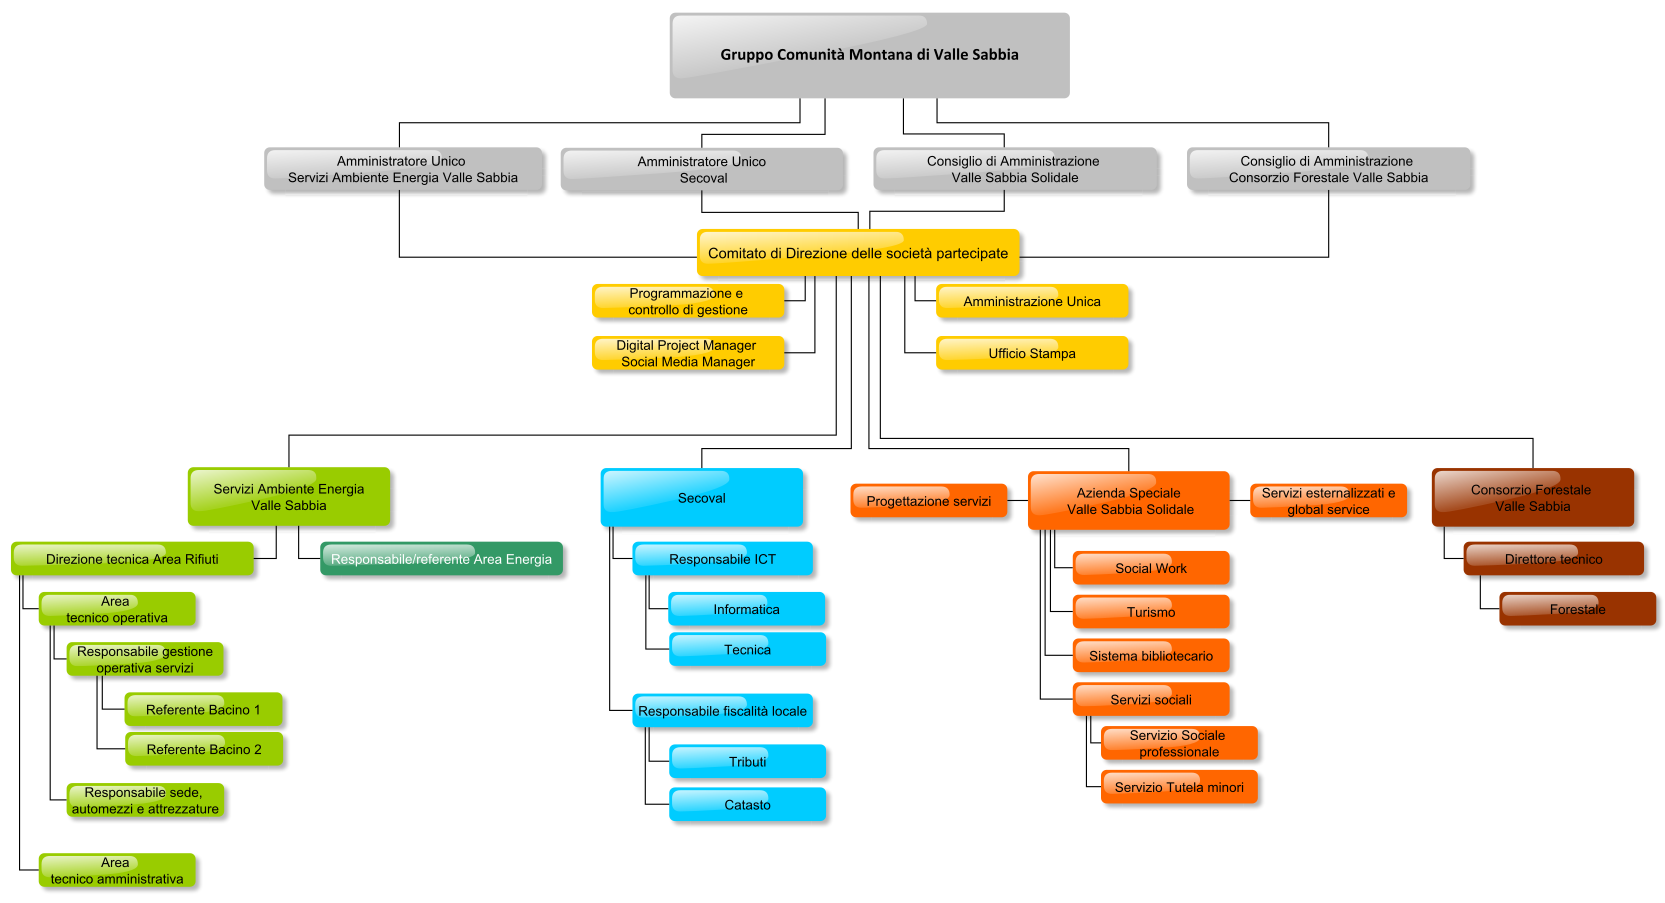
\includegraphics[width=1\linewidth]{figures/organigramma.png}
    \caption{Organigramma Secoval \parencite{organigrammaSecoval}}
    \label{fig:organigramma}
\end{figure}
%DA CONTROLLARE ADD smart city definitions: https://ec.europa.eu/programmes/erasmus-plus/project-result-content/b3c8cbaf-a161-4a99-aaa0-b46a21b1135f/SMACC_Definitions_of_a_Smart_City.pdf
%https://www.ibm.com/think/topics/smart-city
%https://en.wikipedia.org/wiki/Smart_city
Nel contesto tecnologico delle smart city, Secoval gestisce apparati tra cui telecamere per la videosorveglianza urbana (TVCC), Access Point (AP) per la connettività pubblica, switch industriali e gateway LTE per le aree non cablate. Essi fanno parte di reti distribuite sul territorio per l'erogazione di servizi diretti ai cittadini.

Il progetto svolto durante il tirocinio si inserisce direttamente in questo scenario operativo, con l'obiettivo di superare la gestione manuale implementando un'architettura automatizzata e centralizzata basata su Zabbix, in modo che si realizzi un sistema di monitoraggio solido per la rete di apparati di Secoval, abbastanza vasta e appena installata quindi instabile.
Il lavoro ha previsto l'automazione del discovery e dell'assegnazione dei metadati degli apparati tramite fogli Excel, l'integrazione con i flussi di allarme nativi dei dispositivi periferici (come gli eventi ISAPI Hikvision) e la comunicazione sincrona e crittografata con la piattaforma cloud di ticketing aziendale Interacta per la gestione asincrona dei guasti da parte degli operatori.

\section{Il progetto di stage}
Il progetto di stage ha come obiettivo la progettazione e l'implementazione di un'architettura di monitoraggio centralizzata basata su Zabbix 7.0. Esso sarà destinato alla gestione di una delle infrastrutture di rete per smart city che Secoval si trova a gestire. L'esigenza primaria è migliorare e superare i limiti dei sistemi di monitoraggio precedenti, come PRTG (Paessler Router Traffic Grapher), software proprietario con un sostanziale costo per la gestione di reti di certe dimensioni \parencite{PaesslerPricing} e con un'elevata gestione manuale nella implementazione precedente al tirocinio.

L'infrastruttura monitorata è eterogenea e distribuita sul territorio. I dispositivi principali comprendono e si dividono in:
\begin{itemize}
    \item \textbf{Telecamere di videosorveglianza (TVCC):} principalmente telecamere di marca Hikvision, che richiedono il controllo di raggiungibilità e dell'integrità del flusso video.
    \item \textbf{Access Point (AP):} nodi per l'erogazione di connettività pubblica.
    \item \textbf{Switch:} switch industriali, e non, per l'aggregazione del traffico periferico.
    \item \textbf{Dispositivi LTE:} dispositivi delle precedenti 3 tipologie che si basano sull'utilizzo di gateway per l'uplink in aree remote non coperte da fibra ottica.
\end{itemize}

%DA CONTROLLARE FINO A FINE CAPITLO
% Per garantire una gestione flessibile, il progetto fa uso di script esterni (Python e Bash) per espandere le funzionalità native del sistema. Il tradizionale processo di \textit{Network Discovery} basato su ICMP è stato sostituito da un meccanismo di provisioning dinamico via Zabbix API: uno script Python legge un CMDB aziendale in formato Excel e popola automaticamente l'inventario degli host associando l'IP a metadati specifici come l'ID Host, l'ID Palo e le coordinate geografiche. Sul fronte degli eventi, per le telecamere Hikvision è stato sviluppato un middleware Python in ascolto sugli stream ISAPI, incaricato di intercettare alert critici (es. \textit{Video Tampering}) e inoltrarli asincronamente tramite protocollo Zabbix Sender.

% Un requisito fondamentale del progetto è l'integrazione architetturale con \textbf{Interacta}, la piattaforma cloud aziendale per il ticketing. La comunicazione bidirezionale è gestita da un Custom AlertScript eseguito localmente sul server Zabbix, il quale apre e risolve automaticamente i ticket di intervento al variare dello stato dei trigger. La sicurezza di questa comunicazione Server-to-Server è garantita dall'utilizzo di JSON Web Token (JWT) generati e firmati crittograficamente con algoritmo asimmetrico RSA (RS512) tramite librerie Python dedicate.

% A completamento dell'infrastruttura, sono stati integrati strumenti per l'analisi dei dati operativi. Le serie storiche degli allarmi vengono esportate su file system in formato testuale (CSV) ed elaborate da un motore di analisi Python per estrarre Key Performance Indicators (KPI), tra cui il \textit{Mean Time To Resolution} (MTTR) e l'incidenza di anomalie hardware (flapping). L'orchestrazione di questi flussi di esportazione, l'invio della reportistica e la rotazione sicura dei file di log avvengono a livello di sistema operativo Linux sfruttando utilità native come Crontab e Logrotate.

\section{Obiettivi e analisi dei requisiti}
Il progetto formativo mira a trasformare l'infrastruttura di rete (videosorveglianza, Wi-Fi pubblico) che serve 31 Comuni in un sistema smart city che possa essere monitorato e possa scalare facilmente, lavorando su tre pilastri:
\begin{itemize}
    \item[] Sviluppo e miglioramento del monitoraggio di rete.
    \item[] Integrazione degli apparati (telecamere, switch, AP) con la Cartografia GIS per creare uno strumento di gestione georeferenziato.
    \item[] Integrazione con la piattaforma cloud di ticketing aziendale Interacta, garantendo la sicurezza delle comunicazioni machine-to-machine.
\end{itemize}
\begin{figure}[H]
    \centering
    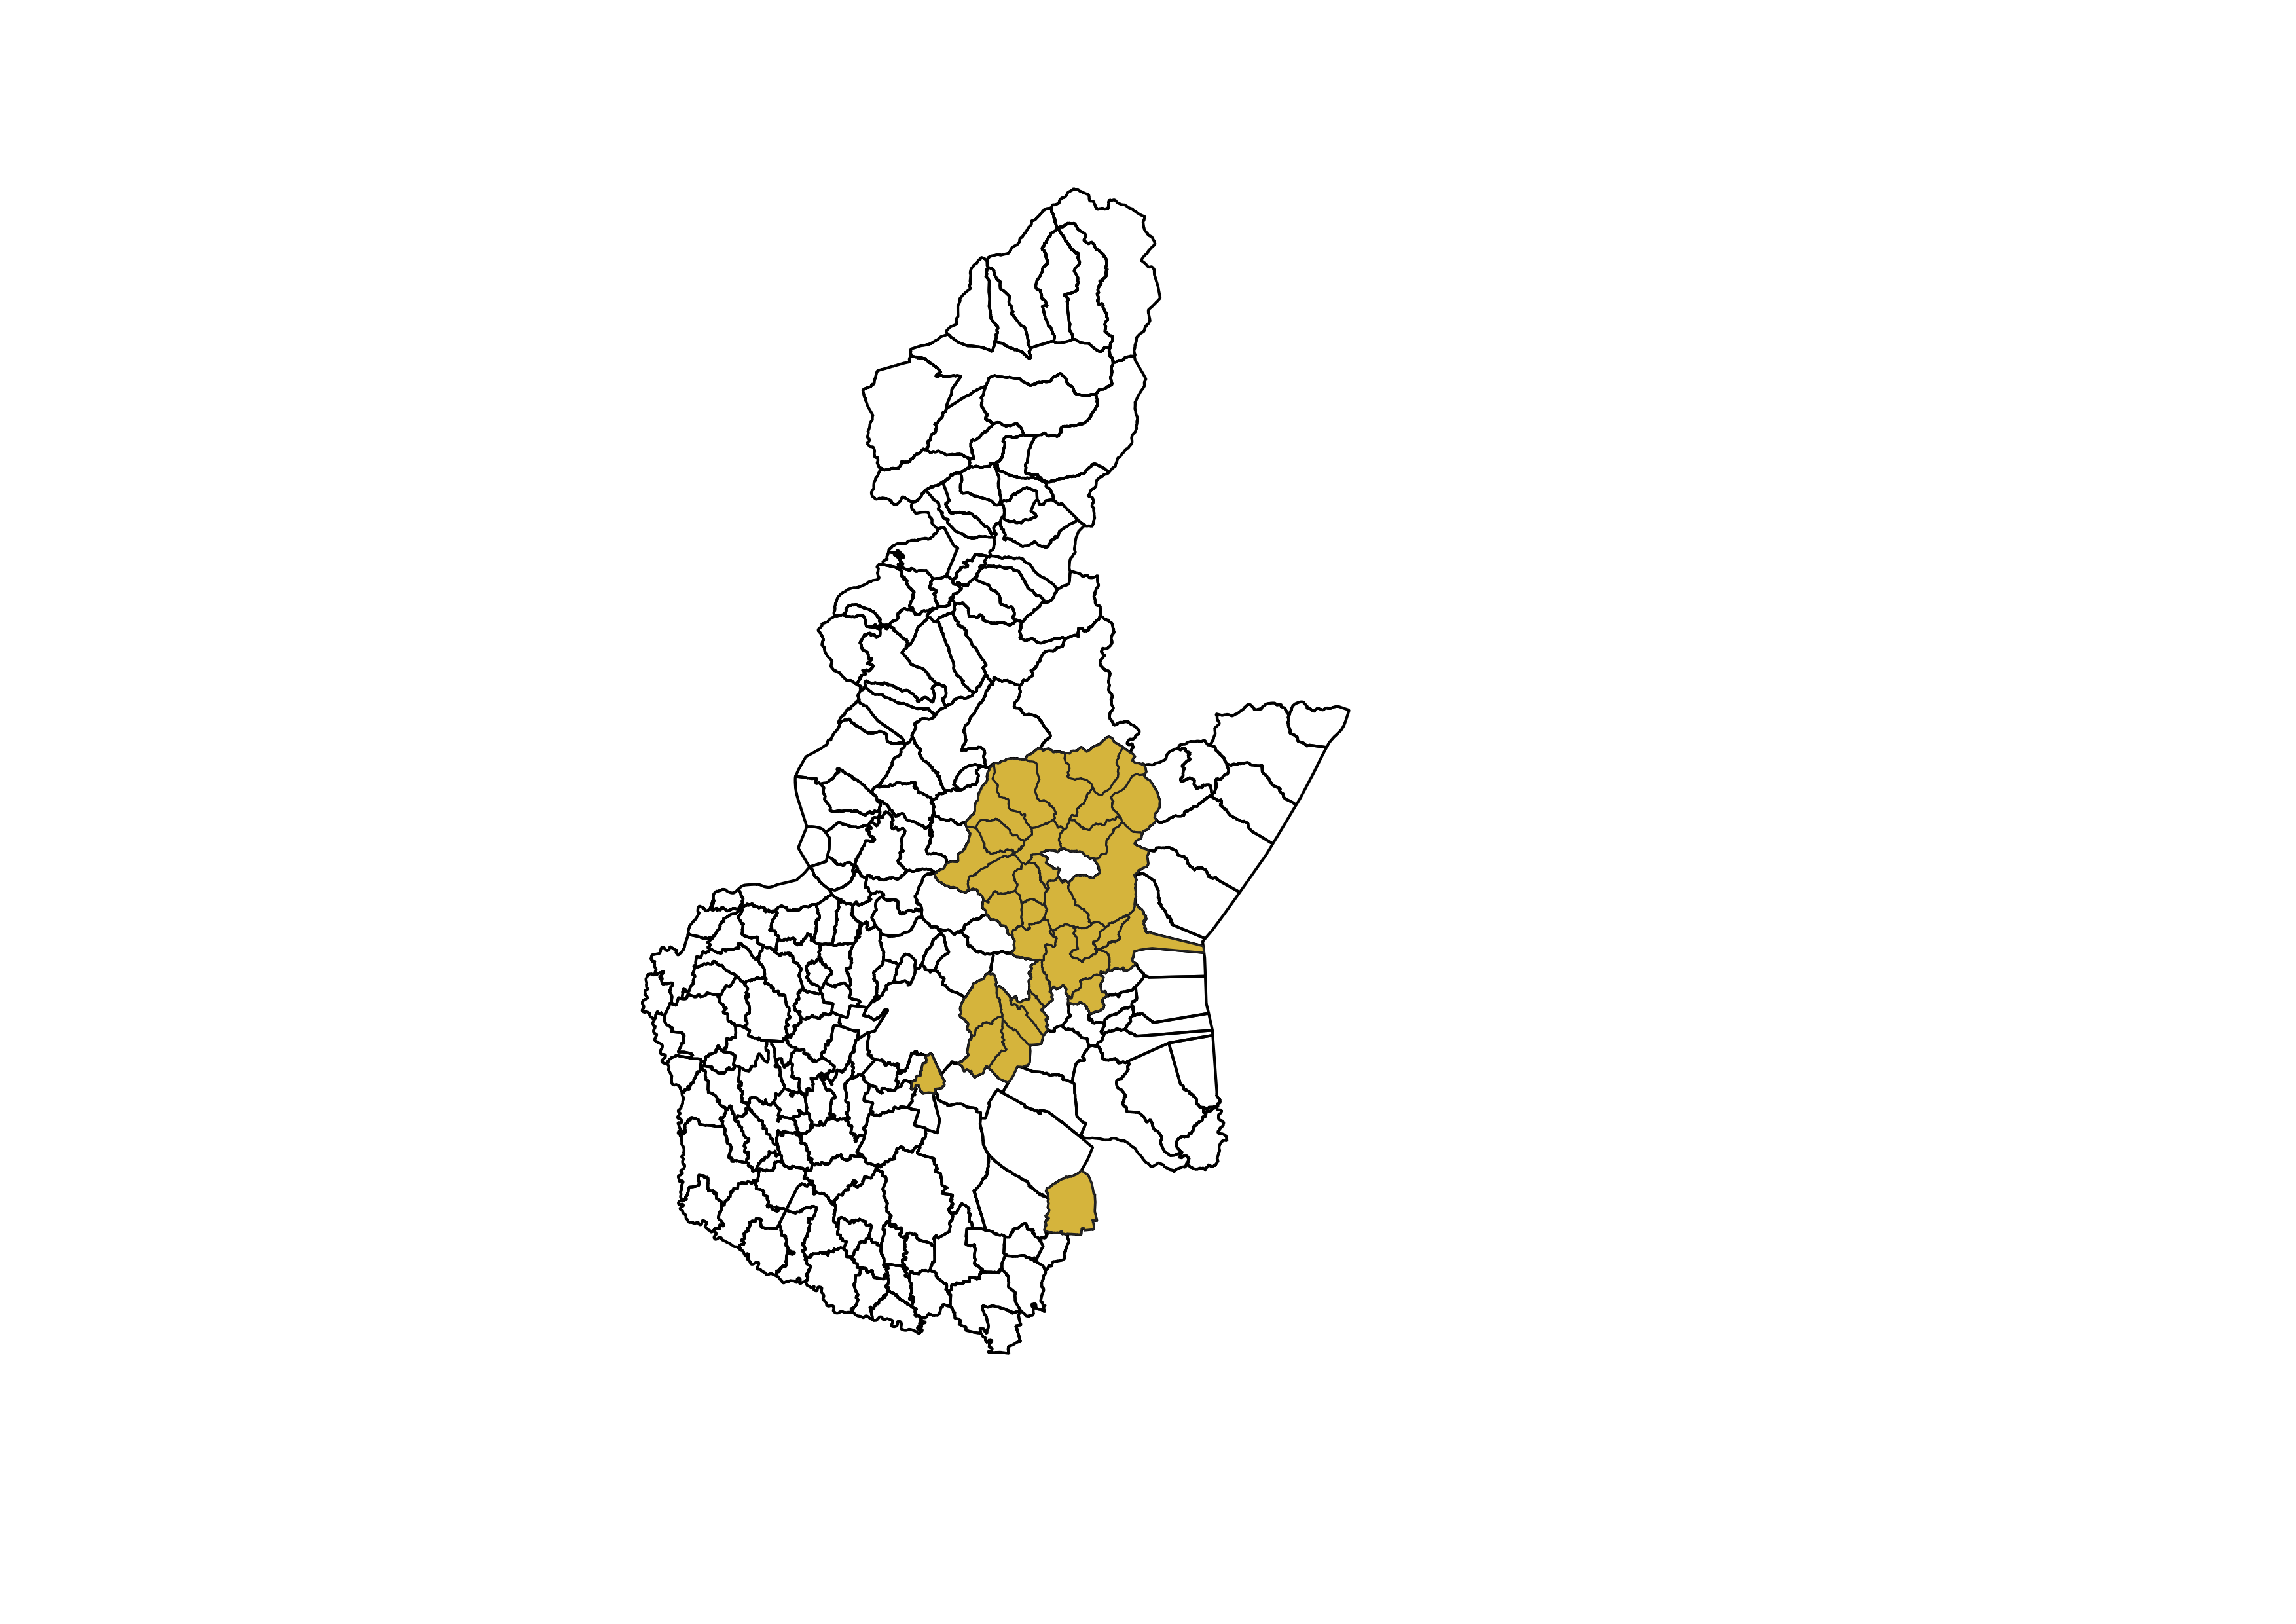
\includegraphics[width=1\linewidth]{figures/ComuniConTelecamere.png}
    \caption{Mappa relativa ai comuni che si avvalgono del sistema smart city}
    \label{fig:ComuniConTelecamere}
\end{figure}

\subsection{Classificazione dei requisiti}
L'analisi del contesto applicativo e dei vincoli imposti dall'infrastruttura e dall'azienda ha portato alla definizione dei seguenti requisiti tecnici e funzionali.

Requisiti:
\begin{itemize}
    \item[] \textbf{Associazione metadati:} attraverso un Configuration Management Database in formato Excel, il sistema deve associare agli host, identificati con gli indirizzi IP, metadati specifici (ID Host, ID Palo).
    \item[] \textbf{Gestione degli eventi TVCC:} il monitoraggio deve intercettare logiche di allarme provenienti dalle telecamere, come il \textit{Video Tampering} e il \textit{Motion Detection}, mediante l'ascolto continuo degli stream ISAPI  e visualizzarli nel frontend di Zabbix.
    \item[] \textbf{Automazione del ticketing (Interacta):} al verificarsi di un disservizio o al suo rientro, il sistema deve interfacciarsi con le API REST del cloud aziendale Interacta per gestire l'apertura e la risoluzione automatica dei ticket. La comunicazione machine-to-machine deve supportare qualche tipo di autenticazione.
    \item[] \textbf{Elaborazione KPI:} il sistema deve estrarre informazioni e metriche riguardo gli host, per offrire anche una visione d'insieme sullo stato del sistema.
\end{itemize}

\begin{figure}[H]
    % Apre l'ambiente per l'immagine. [H] forza l'immagine a stare esattamente QUI (requires \usepackage{float}).
    % In alternativa, usa [htbp] per lasciare che LaTeX trovi la posizione tipografica migliore (Here, Top, Bottom, Page).
    \centering
    % Centra l'immagine orizzontalmente nel foglio.
    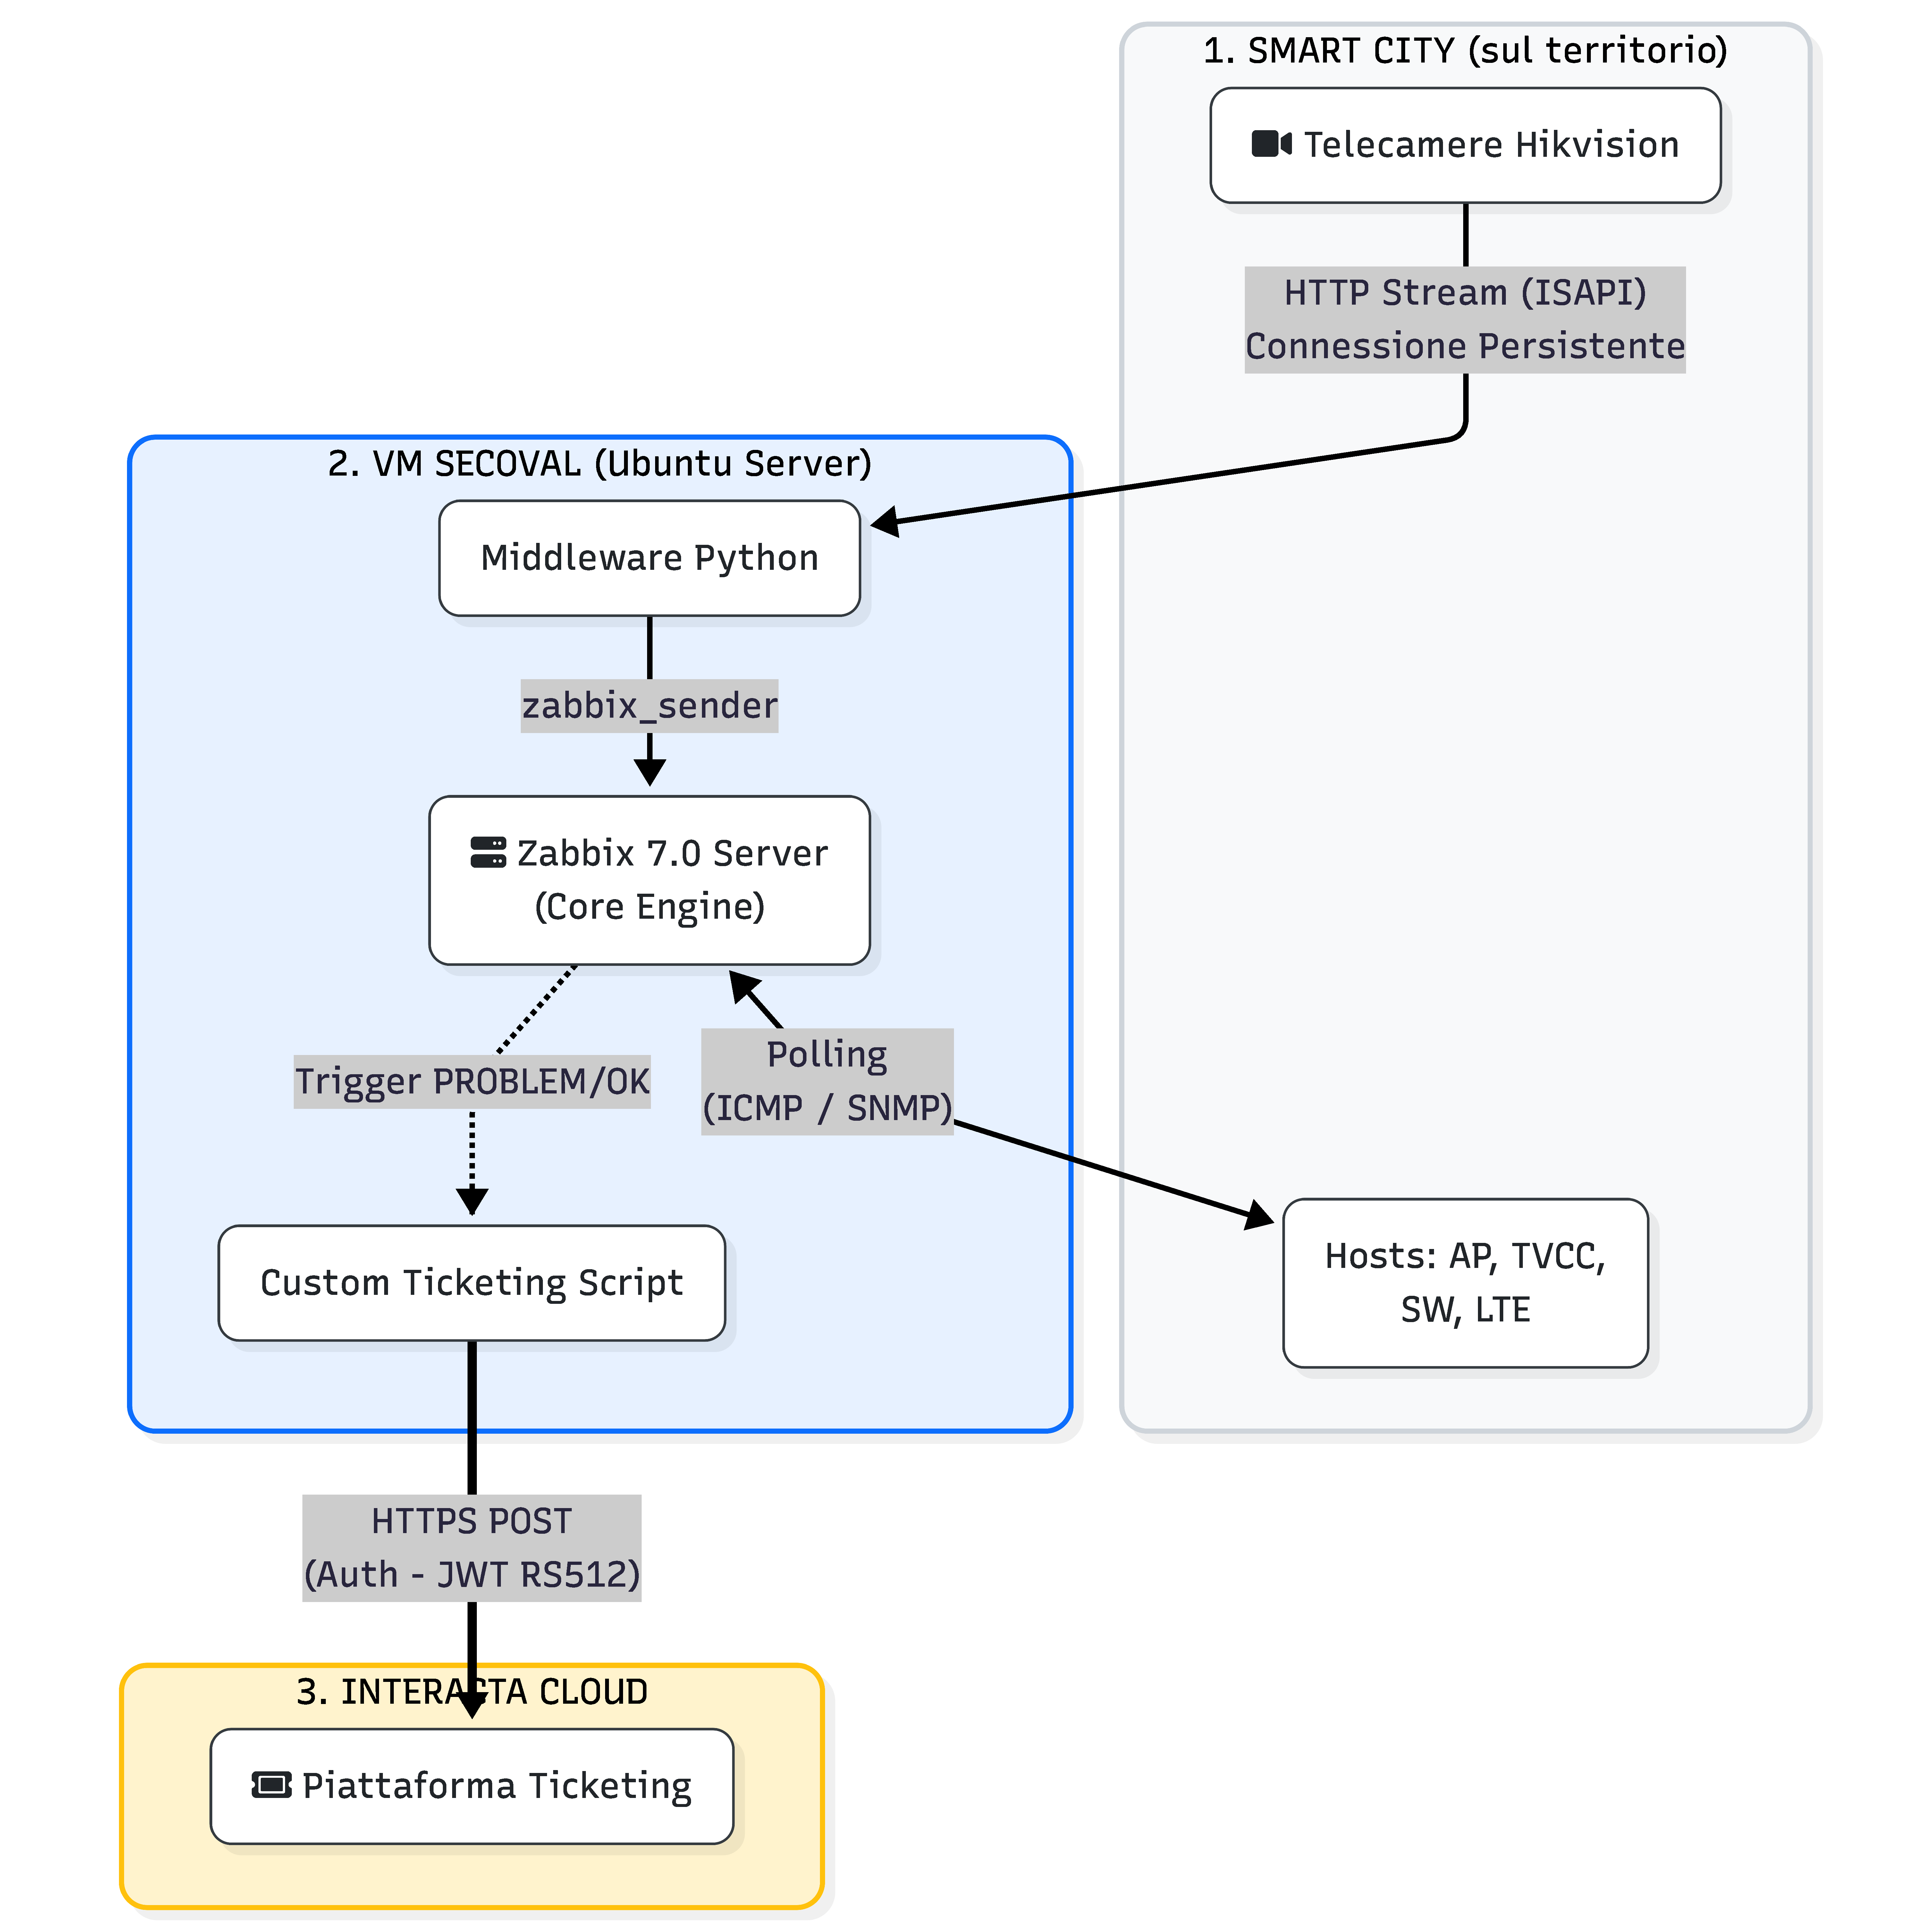
\includegraphics[width=1\linewidth]{figures/SystemArchSchema-2026-06-28-074223.pdf}
    % \includegraphics è il comando "magico" fornito da graphicx.
    % [width=1\linewidth] dice a LaTeX di scalare l'immagine affinché sia larga esattamente quanto la larghezza del testo della pagina.
    % Tra le graffe metti il percorso.
    % TRUCCO PRO: Puoi anche omettere ".pdf" scrivendo solo {figures/SystemArchSchema...}, LaTeX troverà il file automaticamente!
    %\caption{Architettura concettuale del sistema di monitoraggio smart city e flussi di comunicazione.}
    \caption{Schema a blocchi come astrazione del sistema}
    % La didascalia che apparirà sotto l'immagine. Scrivi sempre una didascalia descrittiva in una tesi.
    \label{fig:SystemArchSchema}
    % Il "segnalibro" invisibile. Ti permette di citare l'immagine nel testo scrivendo: "Come visibile in Figura \ref{fig:SystemArchSchema}...".

\end{figure}

\chapter{Tecnologie utilizzate}
\section{Ubuntu Server}
\begin{figure}[h]
    \centering
    
\includegraphics[width=0.3\textwidth]{figures/Ubuntu-logo.png} % Inserire il path corretto
    \caption{Logo Ubuntu}
    \label{fig:ubuntu_logo}
\end{figure}

L' infrastruttura di monitoraggio è stata messa in produzione su una macchina virtuale con sistema operativo Ubuntu Server\parencite{UbuntuServer}. Il sistema operativo mette a disposizione strumenti nativi utili per automatizzare il lavoro in background, rendendo il sitema più robusto e autonomo senza la necessità di appoggiarsi a software di terze parti.

Per orchestrare i flussi di dati e i vari script, il progetto ha sfruttato intensivamente tre componenti e tool di Ubuntu. Il primo è \textbf{Crontab} \parencite{man_crontab}, lo schedulatore di Linux che permette di eseguire comandi a orari o intervalli prestabiliti. È stato utilizzato per gestire le operazioni periodiche. Ad esempio, la generazione e l'invio del report delle statistiche via email prima dell'inizio del turno aziendale.

Il secondo strumento impiegato  è \textbf{Systemd}, ovvero il programma che gestisce i servizi del sistema operativo. Per garantire che lo script Python in ascolto sulle telecamere fosse sempre in funzione, è stato trasformato in un servizio di sistema (demone). Systemd lo avvia automaticamente all'accensione del server e lo riavvia in totale autonomia a seguito di eventuali errori imprevisti o cadute di rete o spegnimenti improvvisi.

Infine, è stata affrontata la gestione dello spazio su disco. Un sistema sempre attivo genera continuamente righe di log; tuttavia, se lasciate accumulare, questi file saturerebbero la memoria. Per prevenire questo rischio, è stato configurato \textbf{Logrotate}. Questa utility di sistema ogni settimana intercetta i file di log, li comprime per ridurne il peso e li archivia.

\section{Zabbix 7.0 LTS}

\begin{figure}[H]
    \centering
    
\includegraphics[width=0.3\textwidth]{figures/Zabbix_logo.png}
    \caption{Logo Zabbix}
    \label{fig:zabbix_logo}
\end{figure}


\hyperlink{glo:Zabbix}{Zabbix} è una piattaforma open-source progettata per il monitoraggio, anche distribuito, e in tempo reale di metriche di rete, apparati, server e applicativi. L'architettura del sistema si fonda su un modello client-server altamente scalabile, composto dai seguenti moduli principali:

\begin{itemize}
    \item \textbf{Zabbix server:} il motore centrale sviluppato in linguaggio C. Si occupa della raccolta dei dati, della valutazione dei \hyperlink{glo:trigger}{\textit{Trigger}} (soglie di allarme) e delle \hyperlink{glo:action}{\textit{Actions}}.
    \item \textbf{Database relazionale:} il livello di persistenza dei dati, tipicamente basato su PostgreSQL o MySQL(MySQL in questo progetto), in cui si archiviano le configurazioni e le serie temporali.
    \item \textbf{Web frontend:} l'interfaccia utente sviluppata in PHP, utilizzata per l'amministrazione del sistema, la configurazione visuale e la generazione di dashboard analitiche. \emph{Apache2} è il web server impiegato in questo progetto.
    \item \textbf{Zabbix Proxy e Agent:} demoni impiegati sugli host periferici limitando il carico sul server centrale e dando la possibilità di distribuire il sistema. Non utilizzati in questo progetto.
\end{itemize}
%DA CONTROLLARE FINO A FINE SECTION
Il funzionamento della piattaforma si basa su due metodi per l'acquisizione dei dati. Il primo è il \textit{polling}, in cui il server interroga ciclicamente i dispositivi tramite protocolli standard come ICMP o SNMP. Il secondo è il \textit{trapping}, che consente a sistemi esterni di spingere i dati verso il server Zabbix. Di questo secondo metodo si avvale l'utility a riga di comando \texttt{Zabbix Sender}.

Per questo progetto è stata adottata la versione 7.0 LTS (Long Term Support) \parencite{zabbix7_Docs}. La scelta di una release LTS garantisce stabilità. Utili dal punto di vista delle attività del tirocinio questa versione include:

\begin{itemize}
    \item \textbf{API JSON-RPC:} l’API web di Zabbix, un'interfaccia strutturata che consente il controllo totale della piattaforma via codice. È stata utilizzata per popolare l'Host Inventory leggendo i metadati dal CMDB aziendale.
    \item \textbf{Custom AlertScripts:} la capacità di lanciare eseguibili esterni (Python, Bash...) al verificarsi di un evento. Questo modulo è stato impiegato per integrare Zabbix con la piattaforma cloud Interacta, e per creare un sistema di logging del sistema.
\end{itemize}

Per facilitare la lettura e la comprensione di questo elaborato si consiglia la lettura delle voci del glossario riguardanti Zabbix. Identificate da: "(Zabbix)".

\section{Python, Venv e i package pip utilizzati}

\begin{figure}[h]
    \centering
    
\includegraphics[width=0.3\textwidth]{figures/Python-logo.png} % Inserire il path corretto
    \caption{Logo Python}
    \label{fig:python_logo}
\end{figure}
%https://commons.wikimedia.org/wiki/File:Python-logo.png

Python \parencite{PythonSoftwareFoundation} è un linguaggio di programmazione ad alto livello, interpretato, tipizzato dinamicamente e orientato agli oggetti. Nel contesto di questo progetto, Python è stato il linguaggio principale utilizzato per estendere le funzionalità di Zabbix e interfacciare ulteriori sistemi.

L'esecuzione degli script all'interno del server Linux si è basata su \texttt{venv} (Virtual Environment). Esso è uno strumento nativo di Python e permette di creare ambienti virtuali isolati per ogni progetto. \texttt{Venv} si assicura che le librerie installate al suo interno non interferiscano con altre librerie di altri progetti o nel sistema operativo, aumentando la sicurezza e facilitando il porting del codice.

La gestione dei pacchetti e delle librerie è stata effettuata tramite \texttt{pip} (Package Installer for Python). Di seguito si riportano alcune librerie impiegate per lo sviluppo dei moduli del tirocinio \parencite{pypi_org}:
\begin{itemize}
    \item \textbf{\texttt{pandas} (e \texttt{openpyxl}):} sono librerie molto diffuse per l'analisi e la gestione dei dati. Nel tirocinio sono state utilizzate per leggere e filtrare i file Excel aziendali (i CMDB) contenenti l'elenco degli apparati. Grazie a queste librerie, il sistema è riuscito a estrarre dai file informazioni per configurare i dispositivi su Zabbix senza alcun inserimento manuale.
    \item \textbf{\texttt{pyzabbix}:} è una libreria creata appositamente per facilitare la comunicazione tra Python e Zabbix. Invece di dover costruire richieste HTTP in formato JSON-RPC, questa libreria fa da "traduttore" semplificando il codice. Nel progetto è stata il motore della configurazione dei dispositivi. Ha permesso agli script di autenticarsi sul server Zabbix tramite API token e di lanciare comandi per creare, aggiornare i dispositivi/host.
    \item \textbf{\texttt{requests}:} è una libreria progettata per inviare richieste HTTP. In questo progetto è servita per inviare i dati verso la piattaforma cloud Interacta.
    \item \textbf{\texttt{PyJWT} e \texttt{cryptography}:} sono librerie dedicate alla sicurezza informatica e alla crittografia. Sono state utilizzate per gestire l'autenticazione tra il server Linux e Interacta. %Nello specifico, hanno permesso di generare e firmare in modo sicuro i token di accesso (JWT) tramite l'algoritmo asimmetrico RS512. Questo passaggio era obbligatorio per ottenere l'autorizzazione a creare i ticket sulla piattaforma.
\end{itemize}

\section{Interacta}

\begin{figure}[H]
    \centering
    
\includegraphics[width=0.3\textwidth]{figures/interacta_logo.png}
    \caption{Logo Interacta}
    \label{fig:interacta_logo}
\end{figure}

Interacta è la piattaforma cloud aziendale adottata da Secoval per la gestione dei processi aziendali e del ticketing\parencite{Interacta}. Nel contesto operativo del progetto, questo software rappresenta il punto di arrivo degli allarmi: quando un apparato sul territorio subisce un guasto o perde la connettività, gli operatori assegnati alla manutenzione ricevono una segnalazione sulla piattaforma Interacta, che potrà tradursi in un intervento di cui ogni step sarà tracciato secondo gli usi aziendali. Durante il tirocinio uno degli obiettivi è stato quello di realizzare l'integrazione, collegando Zabbix direttamente alle API REST di Interacta affinché i ticket di guasto (e i rispettivi rientri) vengano aperti e eventualmente risolti dall'infrastruttura software, rendendo più facile agli operatori la gestione dei guasti.


%DA CONTROLLARE DOVE METTERE QUESTA ROBA
% Trattandosi di una comunicazione \textit{Server-to-Server} tra una macchina virtuale (\textit{on-premise} - \textit{in sede}) e un servizio esterno ospitato sul cloud, l'attenzione si è spostata sulla sicurezza: bisognava impedire a soggetti terzi non autorizzati di poter iniettare finte richieste nel portale di ticketing aziendale. Per risolvere questa criticità, il progetto adotta lo standard \textbf{JSON Web Token (JWT)} \Parencite{JWT}. Un token JWT funziona come un "badge digitale" temporaneo e a prova di manomissione, che accompagna ogni singola chiamata HTTP inviata da Zabbix per dimostrare a Interacta l'assoluta autenticità della comunicazione.

% Per blindare questi certificati digitali, l'infrastruttura sfrutta la crittografia asimmetrica basata sull'algoritmo \textbf{RS512} (chiavi RSA combinate a una funzione di hash SHA-512). Il principio di funzionamento si fonda sulla separazione delle responsabilità: una chiave privata viene custodita gelosamente all'interno del server Linux locale, protetta da permessi rigorosi, mentre la corrispondente chiave pubblica viene depositata sul cloud di Interacta. Al verificarsi di un'anomalia, uno script Python impacchetta i metadati dell'evento, genera un token con una validità temporale di pochi minuti e lo firma digitalmente usando la chiave privata. Quando il pacchetto raggiunge il cloud, Interacta applica la chiave pubblica: se la verifica matematica ha successo, l'identità del mittente è confermata e il ticket viene istanziato sul portale.

\chapter{Architettura e configurazione}
%cosa deve succedere
\section{Setup della macchina virtuale Ubuntu e gestione dei dati}

Per realizzare l'integazione tra i dati Excel e il server Zabbix è stato necessario progettare un ambiente di esecuzione dedicato. L'architettura prevede l'impiego di una Macchina Virtuale (VM) basata su sistema operativo Ubuntu Linux, ospitata sull'infrastruttura di virtualizzazione aziendale (Nutanix). La scelta di Ubuntu Server garantisce stabilità, e  compatibilità con software open-source come Zabbix.

\subsection{Setup della VM Ubuntu}
L'applicativo Zabbix viene eseguito su una virtual machine sui server Secoval, chiamata
"SECZABBIX-TLC". Il sistema operativo utilizzato è Ubuntu Server (Ubuntu 24.04).

Nella VM a livello di sistema operativo, sono stati definiti contesti di esecuzione separati per necessità tecniche:
\begin{itemize}
    \item l'utente \texttt{administrator}: impiegato per le fasi di sviluppo, l'utilizzo di SSH e per l'aggiornamento dei file Excel di input. La maggior parte della \textit{codebase} risiede all'interno della sua directory di lavoro, specificamente nel percorso \\\texttt{/home/administrator/zabbixHostsScript/}.
    \item l'utente di sistema \texttt{zabbix}: utilizzato dal demone del server di monitoraggio per l'esecuzione in background degli script di alert e di integrazione.
\end{itemize}

\section{Zabbix nella funzione di monitoraggio della smart city}
\subsection{Architettura generale dell'infrastruttura}
L'infrastruttura che necessita di monitoraggio nel progetto di \emph{smart city}
è costituita da una serie di sottoreti virtuali \emph{VLAN} che si sviluppano sul territorio. In esse sono collegati diversi host, di natura eterogenea,
per oltre 1000 dispositivi attivi.

Come già discusso in precedenza, il monitoraggio delle sottoreti era affidato a Paessler PRTG Network Monitor.
La migrazione a Zabbix è stata una scelta dettata da fattori di costo e anche di automatizzazione: le API di Zabbix sono
più facilmente utilizzabili e meglio documentate, per la loro natura open-source.

Per ogni comune si possono avere 4 sottoreti, per esempio nel comune di \lstinline|Lavenone|:
\begin{description}
    \item [TVCC-LAVE:] ne fanno parte le telecamere principalmente di marca Hikvision, un gateway e un possibile server di gestione delle telecamere da parte del comune.
    \item [SW-LAVE: ]ne fanno parte gli switch, un gateway e un possibile server.
    \item [AP-LAVE: ]ne fanno parte gli access point e un gateway.
    \item [LTE-LAVE:] sottorete facoltativa che contiene host di ogni tipo che si basano su
          tecnologia LTE o satellitare per comunicare da aree remote non coperte dai normali servizi.
\end{description}

La \textbf{funzionalità principale del sistema} consiste nell'applicare in Zabbix il template \emph{ICMP ping}
ad ogni host presente nelle VLAN del progetto.
Questo template permette lanciare verso tutti gli host un comando \emph{ping} ogni minuto e misurare,
tra 3 diversi item, l'accessibilità dell'host sulla rete. In caso di comunicazione interrotta
il relativo trigger lancia un problem con \lstinline|Severity: high|.
\subsection{L'autodiscovery degli host da parte di Zabbix}
Essendo le sottoreti da monitorare già presenti nel sistema di monitoraggio precedente, PRTG, con il nome desiderato, è stato esportato
un file \emph{json} contenente un array di oggetti così strutturati:
\begin{lstlisting}[language=c, caption=Struttura della singola sottorete estratta da PRTG]
    {
        "PRTG_ID":  4591,
        "Full_Path":  "smartCity/LAVENONE/TVCC-LAVE",
        "GroupName":  "TVCC-LAVE",
        "IPv4_Subnet":  "x.x.x.x/x"
    },
\end{lstlisting}
Questo file è stato utilizzato per inizializzare in Zabbix le stesse sottoreti,
attraverso uno script python.

In Zabbix gli host possono essere catalogati in \emph{host groups},
a cui vengono assegnati da delle \emph{actions} chiamate \emph{discovery actions}
dopo essere stati scoperti da delle \emph{discovery rules}: sistemi automatici
che trovano gli host presenti in una determinata sottorete.

I compiti svolti da questo script sono stati:
\begin{itemize}
    \item Creazione di un nuovo \emph{host group} per ogni \lstinline|"Full_Path"|
    \item Creazione di una nuova \emph{discovery rule} per ogni \lstinline|"Full_Path"|
          contenente la sottorete IPv4 e la modalità con cui può scoprire nuovi host,
          in questo caso \lstinline|ICMP ping|
    \item Creazione di un nuovo \emph{discovery action} per ogni \lstinline|"Full_Path"| che assegni
          l'host appena scoperto dalla discovery rule al suo host group
          e allo specifico template \emph{ICMP ping}, citato in precedenza( 3.2.1).
\end{itemize}
\section{I fogli di calcolo aziendali}
Una volta scoperti gli host e memorizzati nel database di Zabbix essi sono operativamente funzionanti, ma non contengono alcuna informazione che li riguarda.
Molte delle loro caratteristiche, come nome e l'ID del palo a cui sono montati, non
sono rilevabili dallo stumento software Zabbix perchè non sono state memorizzati sui singoli host.

Per abilitare un'architettura di monitoraggio automatizzata, è stato necessario identificare una \textbf{sorgente della verità}, ovvero un'entità a cui il sistema potesse attingere per allineare il suo stato con lo stato fisico degli asset sul territorio.

Nel contesto della smart city gestita da Secoval Srl, il Source of Truth riguardo gli asset hardware e software che compongono l'infrastruttura della smart city e la configurazione e mappatura dei dispositivi dislocati sul territorio (telecamere IP, Access Point, gateway LTE, switch di rete) è rappresentato da 2 fogli di calcolo Excel: uno fondamentale come archivio e uno di supporto.


\subsection{Struttura e ruolo dei due file Excel aziendali}
Secoval, e le aziende che hanno implementato fisicamente la rete di telecamere sul territorio, gestiscono la conoscenza della propria infrastruttura smart city attraverso \textbf{due file Excel principali}:
\begin{enumerate}
    \item \textbf{Excel degli asset:} questo documento contiene l'inventario di tutti gli asset hardware (come le telecamere, prevalentemente di marca Hikvision) installati nei vari comuni aderenti al progetto. Per ogni apparato sono mappati dati cruciali quali l'indirizzo IP statico, l'univoco \texttt{ID Host} aziendale, il costruttore, il modello e, dato fondamentale per la manutenzione fisica, l'\texttt{ID Palo} che identifica e da un nome alla posizione di istallazione del dispositivo.
          \begin{table}[ht]
              \centering
              % \resizebox adatta la tabella alla larghezza del testo (\textwidth)
              \resizebox{\textwidth}{!}{%
                  \begin{tabular}{llllllllllllcll}
                      \toprule
                      \textbf{Nome Punto} & \textbf{ID Palo} & \textbf{Tipo Apparato} & \textbf{ID} & \textbf{ID Apparato} & \textbf{Marca/Modello} & \textbf{Nome Host/DNS} & \textbf{Indirizzo IP} & \textbf{Netmask} & \textbf{Gateway} & \textbf{Server DNS 1} & \textbf{Server DNS 2} & \textbf{VLAN ID} & \textbf{Indirizzo MAC} & \textbf{Note} \\
                      \midrule
                      % Riga 1 - Esempio Telecamera
                      1\_Sabbio\_1TVCC    & 1\_Sabbio\_1TVCC & Telecamera di contesto & X           & SABB-TVCC-01         & HIKVISION ...          & SABB-TVCC-01           & X.X.X.X               & 255.255.255.X    & X.X.X.X          & X.X.X.X               & X.X.X.X               & XXX              & XX:XX:XX:XX:XX:XX      &               \\
                      % Riga 2 - Esempio Switch
                      1\_Sabbio\_1TVCC    & 1\_Sabbio\_1TVCC & Switch Industriale     & X           & SABB-SW-TVCC-01      & Switch 5 porte         & SABB-SW-TVCC-01        & X.X.X.X               & 255.255.255.X    & X.X.X.X          & X.X.X.X               & X.X.X.X               & XXX              & XX:XX:XX:XX:XX:XX      &               \\
                      \bottomrule
                  \end{tabular}%
              }
              \caption{Tabella Excel degli asset(dati sensibili offuscati)}
              \label{tab:ExcelAsset}
          \end{table}
    \item \textbf{Excel delle coordinate geografiche:} Questo secondo file cataloga e associa gli \texttt{ID Palo} alle coordinate geografiche relative, espresse in latitudine e longitudine in gradi decimali.
          \begin{table}[ht]
              \centering
              % Adatta la tabella alla larghezza della pagina
              %DA CONTROLLARE
              \resizebox{\textwidth}{!}{
                  \begin{tabular}{lccllcllccccc}
                      \toprule
                      \textbf{Comune} & \textbf{Punto} & \textbf{Lotto} & \textbf{Nome Punto} & \textbf{Wifi Punto} & \textbf{Tipo Punto} & \textbf{Tecnologia} & \textbf{Indirizzo} & \textbf{COORDINATE MYGEST} & \textbf{Latitudine} & \textbf{Longitudine} & \textbf{Dec. Latitudine} & \textbf{Dec. Longitudine} \\
                      \midrule
                      % Riga 1 - Esempio con FTTH (cella azzurra)
                      Agnosine        & 1              & 1              & 1\_Agnosine\_1TVCC  & 4\_Agnosine\_WiFi   & TVCC                & FTTH                & Via XXXXX civ. XX  &                            & 45°XX'XX.X''N       & 10°XX'XX.X''E        & 45.XXXXXX                & 10.XXXXXX                 \\
                      % Riga 2 - Esempio con FWA (cella gialla e testo in grassetto)
                      Agnosine        & 6              & 1              & 6\_Agnosine\_1TVCC  &                     & TVCC                & FWA                 & Via XXXXX          &                            & 45°XX'XX.X''N       & 10°XX'XX.X''E        & 45.XXXXXX                & 10.XXXXXX                 \\
                      \bottomrule
                  \end{tabular}%
              }
              \caption{Tabella Excel delle coordinate geografiche(dati sensibili offuscati)}
              \label{tab:ExcelCoordinate}
          \end{table}
\end{enumerate}

Questi due file sono depositati all'interno del file system della macchina virtuale Ubuntu Server dedicata al monitoraggio, all'interno della directory di lavoro del progetto \\(\texttt{/home/administrator/zabbixHostsScript/}). Essi vengono aggiornati periodicamente dal personale tecnico di Secoval non appena un nuovo apparato viene installato o censito sul campo.



\subsection{L'estrazione dei dati}
Purtroppo Zabbix non è in grado di leggere nativamente un file \texttt{.xlsx} per configurare i propri host. Per risolvere questo problema e automatizzare il flusso di informazioni verso Zabbix, è stato scritto uno sript Python.

Il sistema opera secondo una logica basata su due fasi:
\begin{itemize}
    \item \textbf{Estrazione:} lo script Python, sfruttando  librerie dedicate alla manipolazione dati come \texttt{pandas}, accede ai percorsi assoluti dei due file Excel e ne legge le righe. Questa operazione permette di estrarre la conoscenza testuale racchiusa nelle celle (indirizzi IP, ID Palo, denominazione del Comune). I dati grezzi estratti dagli Excel vengono mappati all'interno di dizionari Python. %In questa fase, ad esempio, lo script associa a ciascun dispositivo il corretto \textbf{Host Group} di Zabbix (es. separando logicamente il gruppo \texttt{SmartCity/TVCC} dal gruppo \texttt{SmartCity/Connectivity}) e determina quale \textbf{Template} di monitoraggio applicare in base al modello hardware rilevato nel foglio elettronico.
    \item \textbf{Caricamento via API:} i dati vengono inseriti all'interno del server Zabbix. Lo script Python effettua chiamate al server zabbix attraverso la libreria \emph{pyzabbix}. Il sistema esegue un confronto tra le informazioni presenti negli Excel e quelle su Zabbix; per esempio se l'IP di un asset non è presente su Zabbix allora non viene forzata la sua creazione, se invece è presente si associano ad esso i relativi metadati(nome, ID palo, coordinate...).
\end{itemize}

\section{Implementazione dell'aggiornamento degli host}

Ogni host in Zabbix viene identificato con un attributo "name" che contiene l'IP con cui è stato scoperto.
Inoltre possiede anche un attributo "visible name" che lo rappresenta nel sistema. L'obiettivo è andare a estrarre
dal file Excel degli asset l'informazione del loro identificativo aziendale, da inserire nell'attributo "visible name"
e l'informazione sull'id del palo su cui sono montati, da inserire le campo "location" del loro attributo
"inventory" (ogni host possiede un ampio elenco di campi da compilare nell'attributo "inventory").

Oltre a queste informazioni, per ogni host è necessario associare anche le coordinate geografiche del palo su cui sono montati.
% Nel file Excel delle coordinate geografiche: viene associata all'IDpalo anche le coordinate geografica.
% Quindi per ogni host con uno specifico IDpalo gli si deve associare anche le coordinate geografiche.

Siccome la quasi totalità delle sottoreti al momento del mio tirocinio
presenta numerosi host con svariati problemi, che impediscono al sistema di scoprirli tramite
ping, risulta impossibile assegnare i loro metadati in una sola volta.
Quindi, mano a mano che essi andranno online, verranno scoperti dal sistema che dovrà associare
a essi le informazioni contenute nei file Excel. Proprio come per gli host scoperti inizialmente.

Questo implica che l'assegnazione di questi dati deve essere fatta periodicamente,
con un periodo congruo. Per questo ho scelto di utilizzare script python, eseguiti periodicamente
dal servizio \texttt{crontab} \parencite{man_crontab} presente nativamente in Ubuntu. Il periodo scelto è di un'ora, in modo da non sovraccaricare il server Ubuntu ma di rendere possibile agli operatori vedere i cambiamenti nella stessa giornata lavorativa.

Nella pratica vengono utilizzati degli script python eseguiti nella macchina virtuale che
ospita Zabbix. Tutti gli script ausiliari vengono salvati nella directory
\texttt{/home/administrator/zabbixHostsScripts} (con alcune eccezioni) e tutte le esecuzioni sono svolte nell'ambiente
virtualizzato \texttt{venv} della stessa directory.

\subsection{Associazione dei metadati agli host}
Esistono due script python che si occupano di associare i metadati agli host, uno per l'associazione dei dati attinetni al singolo host proveniente dal file Excel degli asset e l'altro per l'associazione dei dati relativi alle coordinate geografiche del palo identficato con il proprio ID.

In entrambi i casi vengono estratti gli host dal sistema zabbix attraverso la libreria pyzabbix e le API JSON-RPC di Zabbix alla sua base. Gli host vengono confrontati con i dati presenti nei file Excel. Se ci sono incongruenze, gli host vengono aggiornati con le informazioni corrette altrimenti non avvengono modifiche agli host che posseggono già i metadati corretti.


Questi script vengono eseguiti periodicamente ogni ora tramite questi comandi crontab: %inlineCode formatting
\begin{lstlisting}[language=Python, caption=Setup dell'esecuzione periodica in Crontab]
0 * * * * /home/administrator/zabbixHostsScripts/venv/bin/python3 /home/administrator/zabbixHostsScripts/zabbix_HostName_IDpalo_updater.py >> /home/administrator/zabbixHostsScripts/cron_log.log 2>&1

10 * * * * /home/administrator/zabbixHostsScripts/venv/bin/python3 /home/administrator/zabbixHostsScripts/zabbix_palo_location_and_info_updater.py >> /home/administrator/zabbixHostsScripts/cron_log.log 2>&1
\end{lstlisting}


\subsection{Memorizzazione dei messaggi di log}
Gli script python visti fino a ora generano degli output testuali, che andrebbero nello standard output,
ma vengono reindirizzati dai job crontab in uno specifico file di log:
\lstinline|cron_log.log|, ogni scrittura nel file è preceduta dal timestamp e dallo script che la genera.

Per evitare di memorizzare questi dati all'infinito e generare un file di testo gigantesco,
ho utilizzato il sistema \textbf{Logrotate} \parencite{man_logrotate}, una utility Linux il cui scopo è la rotazione,
compressione e rimozione di file di log automatici.

In questo caso il file contenente le configurazioni per il job logrotate del file \lstinline|cron_log.log| è accessibile nel file: \inlinecode{/etc/logrotate.d/zabbix_scripts}.
Al suo interno troviamo:
\begin{lstlisting}[language=python, caption=Configurazione logrotate per un file di log]
#path del file di log da gestire
/home/administrator/zabbixHostsScripts/cron_log.log {
    #user privileges
    su administrator administrator
    #periodo temporale di rotazione dei log
    weekly
    #quante copie di log tenere
    rotate 12
    #aggiungi la data al nome del file
    dateext
    dateformat -%Y-%m-%d
    #dove archiviare i log
    olddir /home/administrator/zabbixHostsScripts/storico_log
    #comprimi i file di log vecchi ma aspetta un ciclo
    compress
    delaycompress
    #ignora gli errori se il file non esiste
    missingok
    #non ruotare il log se e' vuoto
    notifempty
    # crea un nuovo file alla rotazione e assegna questi permessi 
    create 0644 administrator administrator
}
\end{lstlisting}

\section{Georeferenziazione e GIS integrato in Zabbix}
I metadati associati agli host in Zabbix, come longitudine e latitudine, vengono utilizzati nativamente dal software \hyperlink{glo:GIS}{GIS}(geographic information system) integrato.
Le coordinate geografiche degli apparati vengono estratte dai campi \texttt{location\_lat} (Latitudine) e \texttt{location\_lon} (Longitudine) dell'inventory degli host.
All'interno del widget \emph{GeoMap}, nativamente disponibile nelle dashboard di Zabbix grazie allo stumento OpenStreetMap \parencite{OpenStreetMap}, si possono visualizzare gli host su di una cartina, codificati tramite colore per la gravità dei problemi che eventualmente riscontrano. Essi mantangono l'integraaione con il sistema di monitoraggio, quindi un host con un problema visualizzato in rosso sulla mappa permette di risalire al suo nome e caratteristice e, se risolto, diventa verde in tempo reale.
%DA CONTROLLARE LE FOTO
\begin{figure}[H]
    \centering
    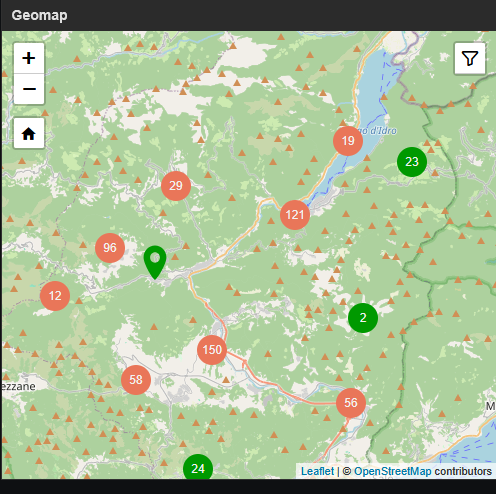
\includegraphics[width=0.5\textwidth]{figures/MapWithProblems.png} % Inserire il path corretto
    \caption{GIS integrato in Zabbix}
    \label{fig:GIS_Zabbix}
\end{figure}
\begin{figure}[H]
    \centering
    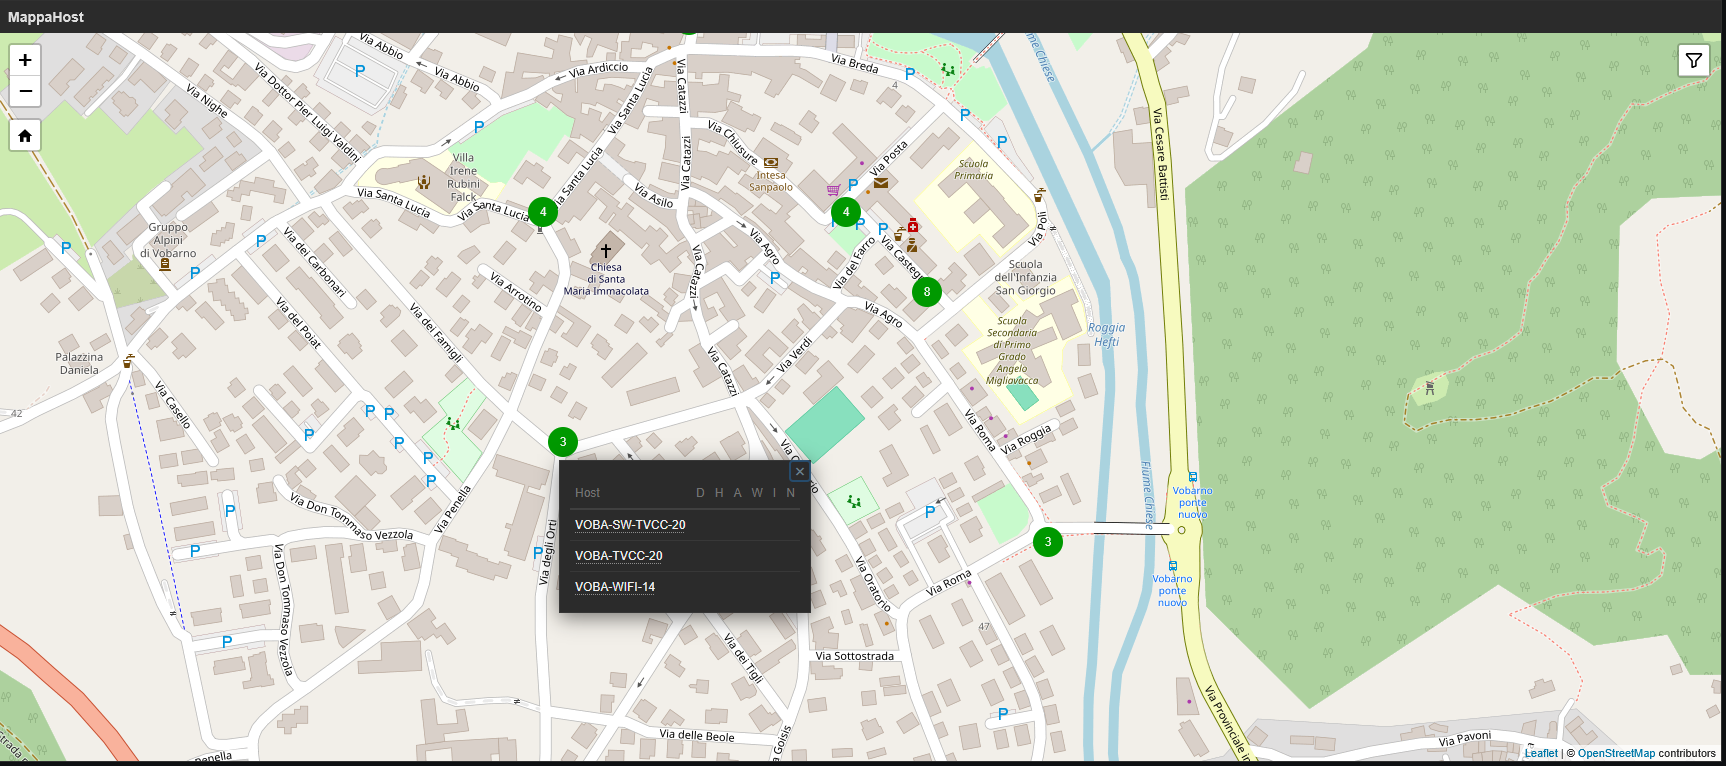
\includegraphics[width=1\textwidth]{figures/MapCloseUp.png} % Inserire il path corretto
    \caption{GIS integrato in Zabbix - dettaglio di un'area}
    \label{fig:GIS_Zabbix_dettaglio}
\end{figure}

\section{Reportistica e KPI}
L'implementazione di un sistema di monitoraggio centralizzato vista fino ad ora genera parallelamente dei dati. Per trasformare questa raccolta di allarmi in informazioni utili al
management aziendale, è necessario estrarre e analizzare le serie temporali.
Poiché Zabbix non supporta nativamente l'invio programmato di file arbitrari o analisi testuali complesse via email, è stata progettato un sistema per il salvataggio dei dati relativi agli eventi rilevati da Zabbix e un sistema per la generazione di report automatici.


\subsection{Esportazione dati evento tramite custom AlertScript}
Per ottenere l'esportazione degli eventi e dei relativi metadati degli host coinvolti, si è deciso di sfruttare il sistema di \textit{Media Types} di Zabbix. Si è intrapresa questa strada invece di una interrogazione diretta del database MySQL di Zabbix per via dei vincoli temporali del tirocinio e per avere flessibilità di elaborazione diretta dei dati tramite le librerie Python.
Solitamente, un Media Type definisce il canale di consegna di una notifica (es. Email, SMS o Telegram). Nel nostro caso, è stato creato un Media Type personalizzato di tipo \textbf{Script}.

A questo Media Type è stata agganciata un'\textit{Action} configurata per scattare ogni volta che si verifica un problema sulla rete smart city. Invece di inviare una mail, Zabbix esegue lo script Bash \texttt{ScriptCustomExportProblemsToCSV.sh} depositato sulla macchina virtuale Ubuntu.

Zabbix passa allo script una stringa contenente tutte le \textbf{Macro} necessarie per l'analisi: i metadati relativi all'host coinvolto. Alcuni parametri in ingresso includono:
\begin{itemize}
    \item \texttt{\{EVENT.ID\}}: identificativo univoco dell'allarme.
    \item \texttt{\{EVENT.DATE\}} e \texttt{\{EVENT.TIME\}}: timestamp di inizio del disservizio.
    \item \texttt{\{EVENT.RECOVERY.DATE\}} e \texttt{\{EVENT.RECOVERY.TIME\}}: timestamp di risoluzione.
    \item \texttt{\{HOST.NAME\}} e \texttt{\{INVENTORY.LOCATION\}}: riferimenti al dispositivo e alla sua ubicazione fisica (es. ID Palo).
\end{itemize}

\subsection{Salvataggio locale in CSV}
Lo script Bash sulla VM Linux riceve l'intera stringa di parametri e provvede ad accodarla al file CSV di destinazione.

\begin{lstlisting}[language=bash, caption=Custom bash script per l'esportazione in CSV]
#!/bin/bash

LOGFILE="/var/log/zabbix/ExportedProblemsToCSV.csv"

# Se il file non esiste crealo e imposta la riga di intestazione
if [ ! -f "$LOGFILE" ]; then
    echo "Status,EventID,Date,Time,Host,IP,Severity,EventName,TriggerName,RecoveryDate,RecoveryTime,Duration" > "$LOGFILE"
fi

# Appendi i dati provenienti da Zabbix 
echo "\"$1\",\"$2\",\"$3\",\"$4\",\"$5\",\"$6\",\"$7\",\"$8\",\"$9\",\"${10}\",\"${11}\",\"${12}\"" >> "$LOGFILE""
\end{lstlisting}

\subsection{Elaborazione dati e report}
Per estrarre significato dai dati immagazzinati che sia utile al team di manutenzione e alla direzione aziendale ho implementato ed eseguito tramite \textbf{Crontab} due diversi tipi di report inviati via mail.

\subsubsection{Report giornaliero}
Il primo è un report giornaliero in cui ogni mattina vengono analizzate le entrate delle 24 ore precedenti. Le informazioni vegono divise in quattro sezioni che anranno a comporre il corpo dell'email:

% Per esempio dei report giornalieri con: il totale dei problemi rilevati il giorno precedente, come si dividono nelle 4 tipologie di sottoreti, i problemi non ancora risoltosi automaticamente che necessitano di attenzione, gli host con oscillazioni, e gli allarmi di oscurazione degli obiettivi.
% Per esempio dei report mensili con: il numero di host attivi sul sistema, in che percentuale di problemi vengono da qualce tipologia di sottoreti, la classifica degli host più problematici, e una analisi temporale della frequenza dei guasti per fascia oraria e per settimana.
\begin{itemize}
    \item \textbf{Riepilogo:} conteggio totale dei problemi rilevati e di quelli risolti automaticamente
          (riconciliando le righe tramite \texttt{EventID}).
    \item \textbf{Problemi non risolti:} una lista degli host che hanno registrato uno stato
          \texttt{PROBLEM} senza un corrispondente \texttt{RESOLVED} nello stesso intervallo di tempo.
    \item \textbf{Infrastruttura instabile (oscillazione):} vengono contate quante volte un host ha attivato un allarme.
          Se il conteggio supera una soglia definita (es. 2 disconnessioni in un giorno),
          l'host viene evidenziato come "instabile".
    \item \textbf{Allarmi di sicurezza critici:} come vedremo in seguito oltre alla disconnessione il sistema può rilevare anche altri allarmi: se presenti, vengono messi in risalto per richiedere un approfondimento immediato.
\end{itemize}
\subsubsection{Report mensile}
Il secondo è un report mensile nel quale si cerca di estrapolare delle informazioni che possano evidenziare dei pattern nel modo in cui gli eventi si presentano. In modo che si possa analizzare la stabilità dell'infrastruttura e la frequenza temporale in cui si presentano le disconnessioni.
Nel report sono presenti:
\begin{itemize}
    \item \textbf{Volume degli eventi:} conteggio totale dei trigger entrati in stato \texttt{PROBLEM}
          e di quelli risolti (\texttt{RESOLVED}) durante l'intero mese.
    \item \textbf{Conteggio degli host monitorati:} il numero degli host presenti nel sistema in quel moento, in modo da tracciare la crescita dell'infrastruttura con l'aggiunta di nuovi comuni.
    \item \textbf{Analisi delle sottoreti:} suddivisione percentuale e numerica degli eventi problematici per tipologia di sottorete (e quindi di apparato),
          calcolata analizzando il terzo e quarto ottetto degli indirizzi IP (sottoreti TVCC, Switch, Access Point, connettività LTE).
    \item \textbf{Classifica host critici:} identificazione dei 100 dispositivi
          che hanno generato il maggior numero di anomalie.
    \item \textbf{Distribuzione temporale:} mappatura degli eventi per fascia oraria e distribuzione settimanale.
          Questa metrica è utile per identificare pattern di disservizio legati a momenti specifici della giornata.
\end{itemize}

\chapter{Rilevamento manomissioni TVCC}
%Sistema di rilevazione delle manomissioni e dell'oscuramento e come si integra in Zabbix e i suoi avvisi
Essendo le telecamere di sicurezza oggetto del progetto abbastanza moderne, è stato valutato come utile l'utilizzo dei sistemi di
intelligenza artificiale implementati a bordo per rilevare diversi tipi di eventi che accadono alla singola telecamera.
Tra questi troviamo la possibilità di rilevare l'oscuramento dell'obiettivo della telecamera.
Per sfruttare questa funzionalità è stato creato un sistema di raccolta e invio automatico di avvisi, integrandolo con Zabbix.

\section{Logiche di Polling vs Trapping in Zabbix}

Per comprendere le scelte architetturali adottate durante il tirocinio, è utile analizzare come il server Zabbix operi per la raccolta e l'elaborazione delle metriche. Zabbix si basa sul concetto di \textit{Item}, ovvero la singola unità di dato raccolta da un host. L'acquisizione di questi Item può avvenire seguendo due paradigmi opposti: il \textbf{Polling} (controllo attivo) e il \textbf{Trapping} (controllo asincrono o passivo).

Per la parte relativa al monitoraggio dell'accessibilità degli host alla rete e al corretto funzionamento dei servizi, è stato utilizzato il paradigma del Polling. Invece per il rilevamento delle manomissioni delle telecamere è stato utilizzato il paradigma del Trapping, in quanto le telecamere Hikvision implementano un sistema di avvisi automatici che possono essere intercettati e gestiti da Zabbix e da script ausiliari.
\section{Descrizione dell'implementazione}
Il sistema gestisce 2 eventi provenienti dalle telecamere: il  tamperdetection o l'oscuramento dell'obiettivo e il motiondetection o il rilevamento di movimento.
Il secondo è stato implementato solo per motivi di debug, dato che condivide gli stessi canali dell'oscuramento ma è molto più facilmente riproducibile.

Il workflow che viene eseguito per garantire la corretta gestione di queste informazioni si divide in questi step:
\begin{itemize}
    \item Estrazione degli IP delle telecamere Hikvision presenti in Zabbix con uno script python.
    \item Ogni IP estratto è utilizzato per lanciare verso la telecamera le configurazioni dei loro servizi tamperdetection e motiondetection tramite configurazioni in formato XML.
    \item Si apre una connessione http con ogni telecamera mantenuta perpetuamente aperta in modo asincrono, attraverso uno script python. Su queste connessioni le telecamere comunicano i loro avvisi ed essi vengono comunicati a Zabbix sugli appositi Item dei trigger tramite un API CLI di Zabbix: zabbix\_sender.
    \item All'interno del template relativo alle telecamere Hikvision abbiamo 2 trigger per motiondetection e oscuramento con le loro impostazioni.
    \item I log di questi script vengono gestiti da logrotate \parencite{man_logrotate} salvandoli fino a 3 mesi.
\end{itemize}
\textbf{Bottleneck}: se molti allarmi si attivano contemporaneamente,
lo script python lancia altrettanti script bash e ciò sovraccaricherebbe la CPU.
Se l'utilizzo rimane per il tamperdetection e solo saltuariamente per motiondetection questo non è un problema.



\section{Configurazioni tamperdetection e motiondetection hikvision tramite XML}

Le telecamere Hikvision espongono una API HTTP con autenticazione che permette di modificare le configurazioni e
le impostazioni della telecamera tramite l'upload di file semi strutturati XML.
Essi riguardano il setup delle impostazioni e della modalità di comunicazione per 2 eventi: tamperdetection e motiondetection.
Dopo avere estratto gli IP delle telecamere da Zabbix, lo script python lancia verso ogni telecamera le configurazioni necessarie per abilitare questi eventi.
Esse gestiscono l'attivazione e l'impostazione dell'area dell'immagine in cui la telecamera è
sensibile all'oscuramento o al motion detection e la comunicazione dell'evento triggerato all'\texttt{EventTriggerNotification center} (lancia la comunicazione http).


\section{Sviluppo del middleware e ascolto degli stream Hikvision ISAPI}


È stato creato uno script python in \\\inlinecode{/home/administrator/zabbixHostsScripts/hikvisionOscuramentoScripts}\\\inlinecode{/hikvision_listener_multiplehosts.py}
che si comporta come middleware. Il suo scopo principale è fare da ponte tra le telecamere di videosorveglianza Hikvision e il server di monitoraggio Zabbix,
intercettando gli allarmi in tempo reale e convertendoli valori di item nel sistema Zabbix.

Invece di interrogare continuamente le telecamere (polling),
lo script si mette in "ascolto" continuo sui loro flussi di eventi (streaming),
catturando istantaneamente anomalie come il rilevamento del movimento (VMD)
o l'oscuramento della telecamera (Tampering/Shelter alarm).

\subsection{Implementazione del listener}
Lo script si collega tramite API token a Zabbix e, utilizzando la libreria pyzabbix,
estrae tutti gli host e ne salva l'indirizzo IP solo
se l'host in questione è una telecamera di marca Hikvision.
Questo rende il sistema altamente scalabile: se aggiungi una nuova telecamera su Zabbix,
il riavvio successivo dello script la includerà automaticamente.

Per ogni telecamera trovata, viene avviato un "task" indipendente grazie alla libreria asyncio.
Questo permette di gestire decine di telecamere contemporaneamente usando un solo processo leggero,
senza che l'attesa di dati da una telecamera blocchi le altre.
Lo script apre una connessione HTTP persistente (Stream) verso l'endpoint ISAPI della telecamera (/ISAPI/Event/notification/alertStream) \parencite{hikvision_isapi_main}.
In questo canale, la telecamera invia frammenti in formato XML ogni volta che accade qualcosa.
Lo script legge il flusso riga per riga, isola i blocchi XML significativi e li analizza in tempo reale.
Estrae il tipo di evento e il suo stato (se attivo o rientrato).
Quando viene rilevato un evento valido (es. movimento o telecamera coperta), lo script deve avvisare Zabbix.
Per farlo lo script esegue un comando di sistema: zabbix\_sender.
Questo è uno strumento a riga di comando nativo di Zabbix,
progettato specificamente per inviare dati a Zabbix.
Il comando comunica a zabbix l'hostname esatto della telecamera, la chiave dell'allarme
(es. hikvision.motionDetection) e il valore (1 per allarme attivo, 0 per allarme rientrato).

\subsubsection{Items in Zabbix}
Nel template \texttt{templateSC\_configurazione\_hikvision} sono presenti 2 nuovi Item di tipo \emph{Zabbix trapper}:
AllarmeItemOscuramento(key: hikvision.oscuration) e AllarmeItemMotionDetection(key: hikvision.motionDetection). %valutare se togliere prova
Essi sono aggiornati solo dallo script listener con zabbix\_sender.

\subsection{Esecuzione continuativa e log}

Lo script viene configurato come servizio systemd \parencite{man_systemd}, garantendo che si avvii automaticamente all'accensione del server.
Se lo script dovesse bloccarsi per un errore critico, il sistema operativo lo riavvierà automaticamente entro 10 secondi.
È stata inserita una regola che "uccide" e riavvia il servizio ogni 24 ore in modo controllato.
Questo è un mezzo per forzare il sistema a riscaricare la lista aggiornata delle telecamere da Zabbix ogni giorno.
Tutto l'output viene reindirizzato in un file di log gestito da \textbf{Logrotate} \parencite{man_logrotate} su disco per permettere il monitoraggio del corretto funzionamento.

\subsection{Trigger actions e integrazione con Interacta}
Quando un Trigger cambia stato (da \texttt{OK} a \texttt{PROBLEM} o viceversa), entra in gioco il sistema delle  \textbf{Trigger Actions} native. Invece di configurare un'Action per inviare una semplice notifica e-mail, il sistema è statoconfigurato per eseguire un'operazione esecuzione remota di script, puntando al \textit{custom media type: script} denominato \\\texttt{interactaCreateOrSolveTicket}.

La motivazione per utilizzare questo paradigma è la possibilità di iniettare dinamicamente il contesto del guasto all'interno dello script Python. L'Action è configurata per passare allo script degli argomenti tramite le Macro di Zabbix, tra cui:
\begin{itemize}
    \item \texttt{\{EVENT.ID\}}: l'identificativo univoco del guasto, essenziale per correlare la futura risoluzione allo stesso ticket aperto in Interacta in cui sarà chiamato \textit{problem\_ID}.
    \item \texttt{\{HOST.NAME\}} e \texttt{\{INVENTORY.LOCATION\}}: per comunicare alla piattaforma l'ID dell'host e il palo fisico su cui i tecnici dovranno intervenire.
    \item \texttt{\{TRIGGER.STATUS\}}: Il valore che indica allo script se inviare alla piattaforma un payload per la creazione (PROBLEM) o per la risoluzione (RESOLVED) del ticket.
\end{itemize}

\chapter{Integrazione con il sistema di ticketing Interacta}
\section{Scopo e architettura dell'integrazione}

L'implementazione di un sistema di monitoraggio rappresenta solo il primo passo verso l'automazione dei processi IT aziendali. In Secoval, rilevare tempestivamente un guasto tramite Zabbix (ad esempio, l'oscuramento di una telecamera o la caduta di un Access Point) è inutile se l'informazione non raggiunge la squadra tecnica incaricata della manutenzione.

Quindi per garantire l'integrazione con il sistema già presente e il tracciamento della gestione della manutenzione e degli interventi fisici
sugli apparati della Smart City,
si è resa necessaria un'integrazione tra il sistema di monitoraggio Zabbix
e il portale (IT Service Management) \textbf{Interacta}.

L'obiettivo dell'integrazione è automatizzare l'apertura di un ticket di assistenza
(con tutti i dettagli dell'host, le coordinate e il tipo di guasto)
nel momento in cui un trigger di Zabbix entra in stato \texttt{PROBLEM},
e chiuderlo in automatico quando lo stato torna a \texttt{RESOLVED}.

L'architettura si basa di uno \textbf{script Python} operante in \\\texttt{/usr/lib/zabbix/alertscripts/}, incaricato di elaborare i dati e comunicare con le API di Interacta. I dati necessari vengono inoltrati a esso sotto forma di arguments da un \textbf{Media Type} di tipo "Script" configurato su Zabbix. L'\textbf{autenticazione} \textit{Server-to-Server} verso le API di Interacta viene eseuita tramite Service Account (Service Account Authentication è un metodo che consente ad applicazioni, script o macchine virtuali di verificare in modo sicuro la propria identità e interagire con API o servizi cloud senza intervento umano) e firma crittografica asimmetrica (RSA).

I ticket creati non devono essere generici, ma devono contenere metadati utili per i tecnici sul campo (es. l'indirizzo IP, l'ID dell'Host, l'ID del Palo fisico e la descrizione problema).
Se il problema rientra autonomamente, Zabbix deve comunicare a Interacta di risolvere il ticket, evitando alle squadre tecniche uscite a vuoto.


\begin{figure}[H]
    \centering
    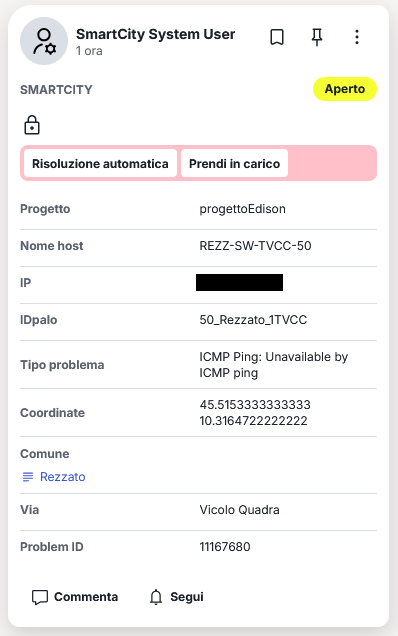
\includegraphics[width=0.5\textwidth]{figures/TicketInteracta.png} % Inserire il path corretto
    \caption{Esempio di ticket in Interacta}
    \label{fig:TicketInteracta}
\end{figure}

\subsection{Autenticazione Server-to-Server}
In un'applicazione web tradizionale, l'autenticazione si basa su interazioni umane (es. inserimento di username e password) e sul mantenimento di una sessione tramite cookie. Nel caso di questo progetto, un server Linux (Zabbix) deve dialogare autonomamente con un altro server (Interacta). Questa modalità \textbf{Server-to-Server}, richiede standard di sicurezza diversi.

La documentazione fornita da Interacta e le linee guida consigliano l'adozione di un'autenticazione basata su token crittografici, specificamente la generazione di una \textit{JWT Assertion}(Json Web Token)\parencite{rfc7519}
firmata con algoritmo \textbf{RS512} utilizzando una chiave privata fornita in formato JSON.

La scelta di questo framework permette di evitare che ci siano \textbf{ credenziali fisse in transito} tramite la generazione di un token JWT "usa e getta" per ogni singolo ticket e singola chiamata HTTPS.
Inoltre permette di garantire lì'integrità, l'autenticazione e il non ripudio delle richieste HTTPS inviate dal sistema.

\section{Generazione e firma del token JWT}

% Il cuore dell'autenticazione verso la piattaforma Interacta si basa sulla costruzione e sulla firma crittografica di un JSON Web Token (JWT). Questo standard (RFC 7519) permette di trasmettere informazioni sotto forma di oggetto JSON in modo sicuro e inequivocabile, eliminando la necessità di memorizzare credenziali fisse a bordo del sistema di monitoraggio.

\subsection{Struttura del Token e scelta dell'algoritmo}
Un JWT standard è composto da tre parti codificate in Base64URL e separate da un punto (\texttt{.}): l'Header, il Payload e la Signature.
L'Header definisce la tipologia di token e l'algoritmo impiegato. Il Payload contiene le asserzioni e le dichiarazioni sull'entità autorizzata (es. l'identificativo del client, l'istante di emissione e il momento di scadenza). Infine, la Signature costituisce la firma digitale, che garantisce l'integrità del dato in transito.

Le specifiche di integrazione dettate da Interacta imponevano l'utilizzo dell'algoritmo \textbf{RS512} per la fase di firma.
A differenza di algoritmi simmetrici, l'RS512 è asimmetrico e prevede l'uso di una coppia di chiavi: una \textbf{chiave privata}, a bordo della macchina virtuale Zabbix, utilizzata dal middleware per firmare il token in uscita, e una \textbf{chiave pubblica}, caricata in precedenza nel cloud di Interacta, utilizzata dal provider per verificare l'autenticità del token.


\subsection{Implementazione in Python}
L'implementazione del sistema di firma è stata realizzata in linguaggio Python, sfruttando la libreria \texttt{requests} per gli scambi HTTPS in sinergia con il modulo \texttt{cryptography} per la gestione sicura delle chiavi RSA.

Il payload è stato configurato, definendo un tempo di scadenza del token (\texttt{exp}) breve, solitamente impostato a 5 o 10 minuti dal momento dell'emissione (\texttt{iat}).

\begin{lstlisting}[language=Python, caption={Snippet Python per la generazione e firma del JWT con algoritmo RS512}]

import uuid      
import jwt        
import json
import base64
import requests
from datetime import datetime
from cryptography.hazmat.primitives import hashes
from cryptography.hazmat.primitives.asymmetric import padding
from cryptography.hazmat.primitives.serialization import load_pem_private_key


def authentication():
    # firma
    try:
        now = int(time.time())

        header = {
            "kid": key_id, 
            "alg": "RS512"
        }

        payload = {
            "jti": str(uuid.uuid4()), # ID: Universally Unique Identifier
            "aud": "injenia/portal-authenticator", #audience: destinatario del token
            "iss": str(client_id), # issuer 
            "iat": now,       # issued at: time
            "exp": now + 600       # expiry: time
        }

        # costruzione delle prime due parti del JWT
        b64_header = b64url_encode(json.dumps(header).encode('utf-8'))
        b64_payload = b64url_encode(json.dumps(payload).encode('utf-8'))

        # la stringa da firmare
        signing_input = f"{b64_header}.{b64_payload}".encode('utf-8')

        # firma Crittografica  con RS512
        private_key_obj = load_pem_private_key(private_key_pem.encode('utf-8'), password=None)
        signature = private_key_obj.sign(
            signing_input,
            padding.PKCS1v15(),
            hashes.SHA512()
        )

        # Token finale
        signed_jwt = f"{b64_header}.{b64_payload}.{b64url_encode(signature)}"
        
    # API request
    try:

        auth_url = f"{API_BASE}/core/auth/create-access-token-by-service-account"
        response = requests.post(
            auth_url,
            headers={"Content-Type": "application/json", "Accept": "application/json"},
            json={"jwtAssertion": signed_jwt}
        )
       
        response.raise_for_status()
        
        data = response.json()
        
        access_token = data['accessToken']
        
        return access_token
\end{lstlisting}
\section{Apertura o chiusura del ticket}
Una volta ottenuto l’access token il passaggio successivo è utilizzarlo per autenticarsi nell'apertura o chiusura dei ticket.
L'interazione tra Zabbix e lo script Python avviene tramite il passaggio di argomenti a riga di comando. In Zabbix il media type: script lanciato dalle trigger actions è configurato per iniettare dinamicamente il valore delle Macro all'interno del comando di avvio dello script.

Lo script elabora i parametri ricevuti (tra cui \texttt{\{EVENT.ID\}}, \texttt{\{HOST.NAME\}}, e \texttt{\{TRIGGER.STATUS\}}) e implementa una logica condizionale per il ciclo di vita del ticket:
\begin{itemize}
    \item \textbf{creazione:} se il \texttt{\{TRIGGER.STATUS\}} è pari a \texttt{PROBLEM}, lo script compila un payload destinato all'endpoint di "richiesta", inserendo nel corpo del messaggio i dettagli dell'host, l'ID Palo e la natura del guasto. L'\texttt{\{EVENT.ID\}} generato da Zabbix viene salvato all'interno del ticket come chiave univoca di correlazione.
    \item \textbf{chiusura:} se il \texttt{\{TRIGGER.STATUS\}} passa a \texttt{RESOLVED}, lo script compila un payload destinato all'endpoint di "chiusura", inserendo nel corpo del messaggio solo l'\texttt{\{EVENT.ID\}} in modo che la piattaforma cloud di Interacta possa identificare il ticket il cui stato deve passare a "Chiuso/Risolto".
\end{itemize}

\begin{lstlisting}[language=Python, caption={Snippet Python per la apertura o chiusura di un ticket}]
def manage_ticket(ticket_data):
    status = ticket_data["status"]
    event_id = ticket_data["problem_ID"]
    
    token = authentication()

    headers = {
        "Content-Type": "application/json",
        "Accept": "application/json",
        "Authorization": f"Bearer {token}"
    }

    # apertura di un ticket
    if status == "PROBLEM":
        url = f"{API_BASE}/extensions/SmartCity/richiesta" 

        payload = {
            "fields": {
                "progetto": ticket_data["progetto"],
                "nome_host": ticket_data["nome_host"],
                "IP": ticket_data["IP"],
                "IDpalo": ticket_data["ID_palo"],
                "tipo_problema": ticket_data["tipo_problema"],
                "coordinate": f"{ticket_data["coordinate_lat"]} {ticket_data["coordinate_lon"]}",
                "via": ticket_data["via"],
                "PROBLEM ID": int(ticket_data["problem_ID"]),
                "comune": findComuneID(ticket_data["nome_host"])
            }
        }

        r = requests.post(url, headers=headers, json=payload, allow_redirects=True)
        r.raise_for_status()

    # chiusura di un ticket
    elif status == "RESOLVED":
        url = f"{API_BASE}/extensions/SmartCity/richiesta/chiusura" 
        
        payload = {
            "clientUid": int(ticket_data["problem_ID"])
        }

        r = requests.post(url, headers=headers, json=payload, allow_redirects=True)
        r.raise_for_status()

    else:
        print(f"Unknown status received: {status}. Expected PROBLEM or RESOLVED.")
\end{lstlisting}


\chapter{Conclusioni}
In questo capitolo vengono presentate le conclusioni del progetto, evidenziando i risultati ottenuti, il livello di soddisfacimento dei requisiti
iniziali e le principali considerazioni maturate durante l'esperienza di
sviluppo.

\section{Raggiungimento degli obiettivi}

Durante lo svolgimento del progetto di stage sono stati completati tutti gli obiettivi stabiliti nella fase di analisi dei requisiti. L'introduzione del sistema di monitoraggio dell'infrastruttura di rete preesistente è entrata in produzione durante gli ultimi giorni della mia permanenza in Secoval. Questo mi ha dato l'opportunità di vedere i primi frutti del mio lavoro ed anche affinare il sistema per essere più adatto all'utilizzo reale.

%tabella
\begin{table}[H]
    \centering
    \renewcommand{\arraystretch}{1.8} % Aumenta l'altezza delle celle per maggiore leggibilità
    \setlength{\arrayrulewidth}{1pt}  % Spessore dei bordi simile all'immagine

    % tabularx con larghezza pari al testo.
    % La colonna X adatta la larghezza automaticamente e va a capo.
    % >{\raggedright\arraybackslash}X allinea il testo a sinistra nelle colonne larghe.
    \begin{tabularx}{\textwidth}{|>{\raggedright\arraybackslash}p{4cm}|c|>{\raggedright\arraybackslash}X|}
        \hline
        \rowcolor{gray!20}
        \multicolumn{1}{|c|}{\textbf{Obiettivo}}                            & \textbf{Valutazione}   & \multicolumn{1}{c|}{\textbf{Commento}}                                                                                              \\
        \hline
        Sviluppo e miglioramento del monitoraggio di rete                   & Raggiunto              & Transizione verso un'architettura automatizzata e centralizzata basata su Zabbix 7.0, configurata per scalare facilmente in futuro. \\
        \hline
        \rowcolor{gray!20}
        Integrazione degli apparati con Cartografia GIS                     & \makecell{Parzialmente                                                                                                                                       \\ raggiunto} & Lo strumento di gestione e monitoraggio georeferenziato è operativo ma risiede all'interno del sistema Zabbix senza avere l'opportunità di un integrazione con programmi più avanzati come QGIS utilizzati in azienda. \\
        \hline
        Integrazione con la piattaforma cloud ticketing aziendale Interacta & Raggiunto              & Implementati script Python per gestire in sicurezza l'apertura e chiusura automatica dei ticket in modalità server-to-server.       \\
        \hline
    \end{tabularx}

    \caption{Riepilogo dei requisiti soddisfatti}
    \label{tab:valutazione_obiettivi}
\end{table}

\section{Limiti del sistema e sviluppi futuri}

Sebbene l'architettura implementata abbia raggiunto gli obiettivi prefissati, e quindi ha ridotto il carico di lavoro manuale per la gestione dell'infrastruttura, sono consapevole che rimangano alcuni aspetti critici sia a livello implementativo che architetturale.
Spesso dovuti a inesperienza e a limiti temporali.

Dal punto di vista implementativo manca un sistema di controllo di versione per il codice. Purtroppo in Secoval non è comune gestire codice e l'importanza di sistemi come git \parencite{git_scm} e github non è stata oggetto di discussione. In futuro inserire il codice in una repository github potrebbe essere un buono strumento per garantire la tracciabilità e la resilienza del codice.
%DA CONTROLLARE inserire fonti con collegamenti git e github

Inoltre non è presente un sistema di manuntenzione dell'ambiente Python.
Le librerie installate non sono tracciate attraverso un file standard \textit{equirements.txt} sono indicato solamente nella documentazione da me redatta e fornita a Secoval.

Il sistema è privo una sezione di troubleshooting: nella documentazione appena citata sono presenti i fixes più comuni a cui mi sono rivolto durante l'implementazione e che pensavo potessero esser utili in futuro. Al momento non è stata fatta una analisi dei tool e delle procedure necessarie in caso di guasti al sistema.

\section{Valutazione Personale}

Il periodo di tirocinio trascorso presso Secoval ha rappresentato una importante tappa nel mio percorso di studi in Ingegneria delle Tecnologie per l'Impresa Digitale, fungendo da ponte tra l'astrazione della teoria e la concretezza dell'ambiente di produzione aziendale.


Il passaggio dallo studio universitario alla pratica in azienda mi ha posto di fronte a problematiche che non pensavo sarebbero state così preponderanti. Mentre all'università spesso si evidenzia la correttezza e gli standard dei processi, in azienda ho dovuto misurarmi con la natura imprevedibile del sistema distribuito ed eterogeneo della rete smart city gestita da Secoval.

Ho toccato con mano come l'eterogeneità di questi sistemi renda molto complesso orchestrare il monitoraggio e richieda ad ogni passaggio dei compromessi tecnici e implementativi.

Inoltre, il dialogo con il personale di Interacta, riguardo gli endpoint necessari per il corretto funzionamento del sistema di ticketing, è stato istruttivo. Ho realizzato come la creazione di sistemi, anche software, sia per la maggior parte discussione e confronto. La parte di interazione tra persone è molto importante per l'efficace realizzazione di qualsiasi progetto.

Infine, sono stato soddisfatto di aver condotto in prima persona l'intero ciclo di vita di questo progetto. È gratificante aver rilasciato un sistema attualmente in produzione e utile nell'immediato. Questa esperienza aziendale mi lascia con una consapevolezza delle mie capacità e sicuramente meno timore nell'affrontare nuove sfide.

\clearpage
\phantomsection % Genera un'ancora ipertestuale manuale all'inizio della nuova pagina
\addcontentsline{toc}{chapter}{Glossario}



\chapter*{Glossario}
\markboth{GLOSSARIO}{GLOSSARIO}

Per facilitare la lettura di seguito vengono definiti i termini tecnici principali,
i protocolli e i concetti architetturali utilizzati nel progetto.
\begin{description}
    \item[\hypertarget{glo:action}Action:] (Zabbix) l'azione automatica che il sistema intraprende quando qualche evento soddisfa alcune condizioni. Può essere relativa ai trigger (\textit{Trigger Action}) o alla scoperta di un nuovo host (\textit{Discovery Action}).
    \item[AP (Access Point):] dispositivo di rete che permette la connessione wireless.
    \item[\hypertarget{glo:api}API (Application Programming Interface):] un'interfaccia o "ponte" software che permette a due sistemi o applicazioni diverse (es. script Python e Zabbix) di parlarsi, passarsi comandi e scambiarsi dati in modo sicuro e automatizzato.
    \item[\hypertarget{glo:apijsonrpc}API JSON-RPC :] (Zabbix) l'API web di Zabbix si basa integralmente sul protocollo JSON-RPC. Qualsiasi operazione eseguibile dall'interfaccia grafica (creazione host, assegnazione template, update dell'inventario) è esposta tramite questo protocollo. Es. il popolamento dell'Host Inventory tramite script Python.
    \item[Asyncio:] modulo nativo di Python per la scrittura di codice concorrente e asincrono single-thread.
    \item[Bash:] interprete di comandi testuale predefinito nei sistemi operativi Unix e Linux, per interagire con il sistema operativo ed eseguire script.
    \item[\hypertarget{glo:comunicazioneasincrona}Comunicazione asincrona:] la comunicazione asincrona non richiede la presenza contemporanea degli interlocutori (es. email, ticket o messaggi su Slack e Dropbox, protocollo MQTT). Consente di gestire i messaggi senza interruzioni e di gestire il proprio tempo.
    \item[\hypertarget{glo:comunicazionesincrona}Comunicazione sincrona:] la comunicazione sincrona avviene in tempo reale (es. chiamate, riunioni su Panopto o Zoom, protocollo HTTP). Le decisioni e la gestione dei messaggi devono essere rapide.
          % \item[CMDB (Configuration Management Database):] database utilizzato da \\un'organizzazione per memorizzare informazioni su hardware e software.
    \item[Crontab:] demone di sistema nei sistemi operativi Unix-like utilizzato per pianificare l'esecuzione di comandi \parencite{man_crontab}.
    \item[CSV (Comma-Separated Values):] formato testuale utilizzato per l'importazione ed esportazione di dati in forma tabellare. Ogni riga rappresenta un record e i campi sono separati da un delimitatore, spesso la virgola.
    \item[\hypertarget{glo:GIS}GIS (Geographic Information System):] sistemi informatici (come QGIS) progettati per acquisire, memorizzare, analizzare e gestire dati georeferenziati. Nel caso di Zabbix permettono di visualizzare gli host(apparati) e il loro stato direttamente su una mappa cartografica.
    \item[Git / Version Control System (VCS):] sistema software progettato per tenere traccia delle modifiche apportate ai file (in particolare codice sorgente) nel tempo, permettendo di ripristinare versioni precedenti e collaborare in team \parencite{git_scm}.
    \item[\hypertarget{glo:host}Host:] (Zabbix) qualsiasi dispositivo fisico o virtuale monitorato dal sistema. Nel nostro caso, una telecamera, uno switch, un Access Point o un router.
    \item[\hypertarget{glo:icmpping}ICMP Ping:] ICMP (Internet Control Message Protocol) è un protocollo di livello di rete utilizzato dai dispositivi per scambiare informazioni di diagnostica e notifica degli errori. L'ICMP Ping è lo strumento diagnostico principale basato su ICMP che invia una richiesta (Echo Request) e attende una risposta (Echo Reply) per verificare la connettività.
    \item[\hypertarget{glo:isapi}ISAPI:] Intelligent Security API, un set di API specifico e proprietario sviluppato da Hikvision. Permette di interrogare e comandare le telecamere in modo diretto tramite protocollo HTTP e di ricevere flussi continui di avvisi di sicurezza.
          %In Hikvision cameras, ISAPI stands for Intelligent Security Application Programming Interface. It is a standardized, HTTP-based communication protocol that allows software, apps, and third-party systems (like Home Assistant or Blue Iris) to interact directly with your camera or NVR.
          %ISAPI utilizes a RESTful (Representational State Transfer) architecture, which is standard across modern web development. Developers send commands using standard HTTP methods (like GET for fetching data, or PUT for saving new settings) accompanied by XML or JSON payloads.
          % \item[Script / Middleware:] un programma (in questo progetto scritto in linguaggio Python)
          %  che funge da intermediario. Si occupa di tradurre, filtrare o trasportare dati da un punto A
          %   (es. file Excel o telecamera) a un punto B (Zabbix).
    \item[\hypertarget{glo:item}Item:] (Zabbix) la singola metrica o il singolo dato raccolto da un Host. Esempi di item sono: la risposta di un comando ping a un host o il tempo di risposta, la risposta ricevuta da un comando, il valore di un sensore fisico o virtuale.
    \item[JWT (JSON Web Token):] standard aperto per la trasmissione sicura di informazioni tra due parti come oggetto JSON \parencite{JWT}.
    \item[KPI (Key Performance Indicator):] metriche quantificabili utilizzate per misurare l'efficacia e i progressi di un'azienda. Consentono di valutare le prestazioni e prendere decisioni basate sui dati.
    \item[Logrotate:] utility di sistema Linux progettata per amministrare sistemi che generano un gran numero di file di log, ruotandoli e comprimendoli \parencite{man_logrotate}.
    \item[Machine-to-Machine:] paradigma di comunicazione in cui dispositivi hardware, sensori o server che scambiano informazioni e avviano azioni in modo autonomo, senza intervento umano.
    \item[\hypertarget{glo:macro}Macro:] (Zabbix) variabili integrate in Zabbix (scritte tra parentesi graffe, es. \\\texttt{\{HOST.NAME\}}) che permettono di inserire dinamicamente il nome, l'IP o altri dati all'interno di svariati campi, per esempio le mail di allarme.
    \item[Middleware:] componente software che funge da intermediario tra applicazioni, sistemi operativi o protocolli di rete diversi, traducendo e facilitando lo scambio di dati.
    \item[Polling:] processo di interrogazione continua e ciclica con cui un sistema verifica lo stato di dispositivi periferici. Nel caso del monitoraggio da parte di Zabbix il server centrale interroga ciclicamente e a intervalli regolari i dispositivi periferici per ottenerne lo stato operativo.
    \item[RS512:] algoritmo di crittografia asimmetrica; RS512 utilizza RSA combinato con la funzione di hash SHA-512 per la firma digitale.
    \item[SMTP (Simple Mail Transfer Protocol):] protocollo standard impiegato per la trasmissione di messaggi di posta elettronica tra server.
    \item[\hypertarget{glo:snmp}SNMP (Simple Network Management Protocol):] il linguaggio standard universale utilizzato dai dispositivi di rete per comunicare il proprio stato di salute e la propria configurazione a un server di monitoraggio centrale.
    \item[\hypertarget{glo:template}Template:] (Zabbix) un modello preconfigurato che contiene un insieme logico di Item, Trigger e regole. Viene applicato a più dispositivi per evitare di configurarli manualmente.
    \item[Trapping:] concettualmente simile all'interrupt, dove un segnale che avvisa il nodo centrale del verificarsi di un evento prioritario, sospendendo temporaneamente la normale esecuzione. Nel caso del monitoraggio da parte di Zabbix è il dispositivo periferico (o uno script) a inviare i dati di allarme al server centrale al verificarsi di un evento.
    \item[\hypertarget{glo:trigger}Trigger:] (Zabbix) una regola logica associata a un Item. Es. la telecamera non risponde al ping per 3 minuti, il Trigger "scatta" e genera un allarme (Problem).
    \item[Troubleshooting:] processo logico in cui si ricerca, identifica e risolve un problema all'interno di un sistema informatico o altro.
    \item[TVCC (TeleVisione a Circuito Chiuso):] sistema di telecamere per la videosorveglianza.
    \item[\hypertarget{glo:Zabbix}Zabbix:] è una piattaforma software open-source per il monitoraggio proattivo di infrastrutture IT, reti, server, macchine virtuali e servizi cloud. Consente di raccogliere, visualizzare e analizzare metriche in tempo reale (come utilizzo CPU, RAM, rete e spazio disco), inviando avvisi immediati in caso di anomalie.
    \item[Zabbix Sender:] utility a riga di comando utilizzata per inviare dati o eventi direttamente al server Zabbix.

          %     \item[Base64URL:] Variante della codifica Base64, progettata specificamente per essere "URL-safe" e sicura per i nomi dei file, sostituendo i caratteri `+` e `/` (problematici nelle URL) con `-` e `\_`, e rimuovendo i caratteri di padding `=`. DA CONTROLLARE e capire cosa è
\end{description}

% \begin{description}
%     % \item[MIB e OID:] Il \textbf{MIB} (Management Information Base) è un dizionario o "mappa"
%     %       che descrive la struttura dei dati di un dispositivo.
%     %       L'\textbf{OID} (Object Identifier) è l'indirizzo numerico specifico all'interno di quella mappa
%     %       (es. \texttt{1.3.6.1.4.1.39165.1.1.0}) che identifica un singolo valore, come il numero seriale.
%     % \item[API REST e RESTful... DA CONTROLLARE:] API che seguono il paradigma REST (Representational State Transfer), consentendo una comunicazione più semplice e scalabile tra i sistemi.
%     % \item[Payload:] in informatica, è il "carico utile" di un pacchetto di dati.
%     % Quando lo script aggiorna Zabbix, il payload è il blocco di testo (solitamente in formato JSON)
%     %  che contiene le vere e proprie informazioni da modificare (es. nome e coordinate dell'host).
%     \item[Crittografia Asimmetrica:] Sistema crittografico che impiega una coppia di chiavi distinte (una pubblica per la verifica/cifratura e una privata per la firma/decifratura) per garantire la sicurezza delle comunicazioni.
%     \item[Demone (Daemon):] Programma eseguito costantemente in background nei sistemi operativi Unix-like, progettato per fornire servizi di sistema o applicativi (come l'ascolto di eventi di rete).
%     \item[REST (Representational State Transfer):] Stile architetturale per lo sviluppo di API nei sistemi distribuiti, basato sull'utilizzo standardizzato dei metodi del protocollo HTTP (GET, POST, PUT, DELETE).


\clearpage
\phantomsection
\addcontentsline{toc}{chapter}{Bibliografia}
% \begin{thebibliography}{9}
%     \bibitem{zabbixdoc}
%     Zabbix LLC, \textit{Zabbix 7.0 Manual}. [Online]. Disponibile su: https://www.zabbix.com/documentation/
%     \bibitem{pythondoc}
%     Python Software Foundation, \textit{Python Programming Language}. [Online]. Disponibile su: https://www.python.org/
% \end{thebibliography}

\printbibliography[title={Bibliografia}]

\clearpage
\phantomsection
\addcontentsline{toc}{chapter}{Ringraziamenti}
\chapter*{Ringraziamenti}
\textit{Innanzitutto desidero ringraziare il mio relatore e tutor universitario Prof. \\Francesco Gringoli per il prezioso e costante supporto durante tutto il percorso di tirocinio e stesura della tesi. La sua competenza e disponibilità sono state fondamentali per la realizzazione di questo lavoro.}
\\
\\
\\
\textit{Un sincero ringraziamento va all'azienda Secoval Srl, che mi ha dato l'opportunità di svolgere il tirocinio curricolare. Un grazie particolare a Alessandro Salice, mio tutor, e al team con cui ho collaborato: lavorare con loro mi ha permesso di crescere sia professionalmente che personalmente.}
\\
\\
\\
\textit{Ringrazio la mia famiglia, che mi è stata di grande supporto e comprensione, rendendo possibile il completamento del mio percorso universitario.}
\\
\\
\\
\textit{Desidero ringraziare anche i miei amici, che pur non condividendo il percorso universitario, mi sono stati vicini con affetto e supporto.}% e allegria nei momenti in cui ne avevo più bisogno.
\\
\\
\\
\textit{Infine, un grazie va ai compagni universitari che nel tempo sono
    diventati amici, con cui ho condiviso momenti di studio e di svago.}
\\
\\
\\
\textit{Brescia, 15 Luglio 2026}
%\hspace{1cm}
\hfill{}
\textit{Brando Calderara}
%\textit{[Spazio dedicato ai ringraziamenti: al Prof. Gringoli, al tutor aziendale in Secoval, famiglia e amici].}
\clearpage
\thispagestyle{empty} % Removes headers and page numbers
\mbox{}               % Inserts invisible content to force page creation
\clearpage

\end{document}

